\documentclass[oneside]{memoir}
\usepackage{microtype}
\usepackage{graphicx}
%\usepackage{subfigure}
\usepackage[table]{xcolor}
\usepackage{subcaption}
\usepackage[all]{nowidow}
% \definecolor{grayish}{rgb}{0.95, 0.95, 0.96}
% \definecolor{corn}{RGB}{233, 210, 135}

% hyperref makes hyperlinks in the resulting PDF.
% If your build breaks (sometimes temporarily if a hyperlink spans a page)
% please comment out the following usepackage line and replace
% \usepackage{icml2021} with \usepackage[nohyperref]{icml2021} above.
\usepackage{natbib}
\newcommand{\cicero}{\abr{Cicero} }
\newcommand{\amr}[1]{\texttt{#1}}
\usepackage{caption,color,fancyvrb}
%\usepackage{code,algorithmic,algorithm}
\usepackage{amsmath,amsthm,amsfonts}
\usepackage{algpseudocode}	% For pseudocode typesetting
\usepackage[colorlinks=true,linkcolor=blue]{hyperref}	% For hyper links
\usepackage{bbm}
\usepackage[T1]{fontenc}
\usepackage{lmodern}
% For CJK usage
\usepackage{CJKutf8} 
\usepackage{ucs} 
\usepackage{tabularx}
\usepackage[encapsulated]{CJK} 
\newcommand{\myfont}{gbsn}
\newcommand{\abr}[1]{\textsc{#1}}
\definecolor{grayish}{rgb}{0.95, 0.95, 0.96}
\definecolor{corn}{RGB}{233, 210, 135}
\usepackage{multirow}

% You need a newsubfloat element to use subcaption
\newsubfloat{figure}

\textwidth = 6.5 in
%\textheight = 9 in
\oddsidemargin = 0.0 in
\evensidemargin = 0.0 in
%\topmargin = 0.0 in
%\headheight = 0.0 in
%\headsep = 0.0 in
%\parskip = 0.2in
\parindent = 0.25in

\def\inv{^{-1}}


\begin{document} 

\begin{titlingpage}
\begin{center}

\textsc{\huge \bfseries {Enhancing Strategic Play with AI: }}\\[0.25cm]
\textsc{\huge \bfseries {Negotiations, Assistance, and Reinforcement Learning}}\\[0.25cm]
 
\emph{A prospectus submitted in partial fulfillment of the degree of Doctor of
Philosophy}\\[5.5cm]

%\textsc{\large DRAFT}\\
%\emph{October 18, 2011}\\[2.0cm]

\emph{Preliminary Oral Examination for}\\
\text{\large Wichayaporn Wongkamjan}\\[2.0cm] % [4.0cm]
\emph{Advisor:} \\
\text{Jordan Lee Boyd-Graber}\\[.5cm]
\emph{Committee Members:}\\
\textsc{<COMMITTEE MEMBER 1>}\\
\textsc{<COMMITTEE MEMBER 2>}\\
\textsc{<COMMITTEE MEMBER 3>}\\[2.0cm]

{\bfseries Department of Computer Science}\\
{\bfseries University of Maryland, College Park, MD 20742}\\
{\bfseries March 3, 2025}

\end{center}
\end{titlingpage}

\thispagestyle{empty}
\setcounter{page}{1}
\setcounter{secnumdepth}{3}

%\doublespacing
\DoubleSpacing

\begin{abstract}

Reinforcement Learning (RL) has been known as a crucial technique to solve decision-making problems. Decade studies mostly focus on optimality in discrete and continuous state-action spaces, maximizing sample efficiency or improving scalability. In recent years, we have witnessed RL in language space where it is first applied to align large language models (LLM) with human preferences. RL appears in a training step which requires human feedback collection to train a human reward model, giving \textit{human} feedback on language model token decisions. Recent studies have discovered that human alignment is not the best option when training LLM agents to solve reasoning tasks, e.g. Math (replace with real datasets). Without training any reward model, task rewards are enough to provide reward signals and improve LLM agents even further in reasoning tasks. 

Though, together with RL, LLM agents can perform as well as humans in multiple decision-making tasks (e.g. Go, Chess), their flaws still exist when there is a need for language for cooperation and social intelligence. Our goal is to explore in complex decision-making and language environments, exploit their (near-)optimal strategies while demonstrating their flaws in languages. Ultimately, we aim to enhance human and artificial intelligence (AI) interactions; improving language in AI to be as close to humans and utilizing AI strengths to guide humans in complex decision-making tasks. 

As AI improves, its strategy is yielding optimality, but a way to be as intelligent in language as humans is yet far. We show evidence that Cicero, the first Diplomacy AI agent that has been trained to be optimal in decision-making and a natural language model components, has been over-claimed that it is \textit{superhuman}. It sure does win over humans with high percentage, however, cooperation in such a competitive setting like Diplomacy is also a key. This requires persuasion and deception skills, in which AI is limited when compared to humans. We then introduce an AI advisory system, PHOLUS, designed to support human decision-making in Diplomacy, demonstrating that AI-generated strategic guidance can bridge the skill gap between novice and experienced agents. Lastly, we leverage counterfactual reinforcement learning to identify deception (CTRL-D) in negotiation. Though the work is under a toy setting like Diplomacy, deception under explicit state and action spaces is hard to be captured by humans, making this as well a challenging problem for AI.   

Building upon these foundational explorations in complex environments like Diplomacy, our proposed work will concentrate on significantly advancing AI’s linguistic intelligence and its integration with strategic reasoning, aiming to improve AI capabilities while fostering human learning. We will enhance strategic AI agents by incorporating LLMs and developing an \textit{explainable} AI framework for strategic communication. Concurrently, we plan to develop an AI-driven strategic advisor capable of providing higher-level, abstract guidance, utilizing LLM fine-tuning process involving both supervised fine-tuning and reinforcement learning from human feedback with task-specific rewards. This research is expected to contribute a high-quality dataset annotated with  reasoning for strategic communication in Diplomacy and to experimentally validate methods for empowering LLMs to generate \textit{context-aware} strategic advice, yielding insights transferable to other domains requiring nuanced human-AI collaboration.

\end{abstract}
%\setstretch{.5}

\SingleSpacing

\newpage
\setcounter{tocdepth}{3}
\tableofcontents

\newpage
\listoffigures

\DoubleSpacing

%%%%%%%%%%%%%%%%%%%%%%%%%%%%%%%%%%%%%%%%%%%%%%
%
% Chapter Break
%
%%%%%%%%%%%%%%%%%%%%%%%%%%%%%%%%%%%%%%%%%%%%%%

\chapter{Introduction}
\section{Motivation: The Evolving Frontier of AI in Complex Social and Strategic Domains}

Artificial Intelligence (AI) has made monumental impacts in navigating complex decision-making setups. From achieving superhuman proficiency in games of perfect information such as Chess \citep{campbell2002deepblue} and Go \citep{Silver2016MasteringTG}, recent research is increasingly deep into domains characterized by imperfect information, multi-agent interactions, and the indispensable role of human language. The advent and rapid evolution of Large Language Models (LLMs) \citep{Brown2020fewshot,Achiam2023GPT4TR} have unlocked capabilities in natural language understanding and generation, seemingly bridging the gap between computational intelligence and human-like communication. However, despite these advancements, the integration of sophisticated strategic reasoning with nuanced linguistic competence, especially in environments demanding social intelligence, remains a challenge.

Current AI systems, even those augmented with LLMs, often exhibit limitations when confronted with the subtleties of human cooperation, negotiation, persuasion, and deception \citep{Wei2022EmergentAO}. Issues such as ``hallucination'' \citep{Ji2022SurveyOH}, lack of robust common-sense reasoning, and brittleness in adversarial social contexts highlight that AI is yet to achieve true human-level parity in these complex communicative settings. This underscores a critical insight: while AI can excel in computationally intensive tasks, such as vast search planning or pattern recognition from massive datasets, its ``social and linguistic intelligence'' often lags. Consequently, rather than aiming for full autonomy in all scenarios, a more pragmatic and fruitful direction involves fostering human-AI cooperation, where AI's analytical strengths complement human intuition and social acuity.

This thesis is situated at this evolving frontier, seeking to explore and enhance AI's capabilities in environments where strategic decision-making is inextricably linked with complex linguistic interaction. The core motivation stems from the observation that while AI can learn optimal strategies in well-defined game-theoretic settings, its ability to effectively use language to achieve strategic goals--to persuade, to build trust, to negotiate, or even to ethically navigate deceptive information--is still in its early stages. This research aims to dissect these challenges, proposing novel frameworks and methodologies to imbue AI agents that already have sophisticated strategies with linguistic intelligence ability.

\section{Diplomacy: A Rich Testbed for AI in Strategic Communication}

To rigorously investigate the confluence of strategy, language, and social intelligence in AI, a suitable experimental environment is needed. The board game Diplomacy emerges as an exceptionally well-suited testbed for this purpose. It is a multi-agent game typically involving seven players, each controlling a major European power in the years leading up to World War I. The objective is to gain control of a majority of ``supply centers'' on the game map, which often necessitates forming and, crucially, sometimes betraying alliances.

Diplomacy's unique characteristics make it an ideal crucible for the research questions posed in this thesis:
\begin{itemize}
    \item \textbf{Multi-Agent Negotiation:} Unlike many games, Diplomacy has no dice or other elements of chance. Its core gameplay revolves around negotiation. In ``press'' variants of the game, players engage in private, free-form natural language communication with one another between game turns. This communication is the primary mechanism for forming alliances, coordinating actions, sharing information (or misinformation), and making threats or promises. The nature of this dialogue presents a significant challenge for AI language understanding and generation.
    \item \textbf{Simultaneous Move Resolution:} After a period of negotiation, all players secretly write down their orders for their units (e.g., move, support, hold, convoy). These orders are then revealed and resolved simultaneously. This mechanic means players must anticipate and counteract others' moves, often based on commitments or deceptions made during the negotiation phase. The success of a strategic plan is thus heavily dependent on the player's ability to predict others' actions, which are themselves influenced by linguistic interactions.
    \item \textbf{Mixed Cooperative and Competitive Dynamics:} While the ultimate goal is individual victory, no player can succeed alone in the early to mid-game. Alliances are essential. This creates a complex interplay of cooperation (within alliances) and competition (against those outside alliances, and eventually, even against former allies). Agents must balance the need to collaborate with the imperative to advance their own position, often leading to situations where trust is built and then strategically broken.
    \item \textbf{The Centrality of Persuasion and Deception:} Effective play in Diplomacy requires social skills. Players must be able to \textit{persuade} others to undertake actions beneficial to them, often by appealing to shared interests, reciprocity \citep{kramar2022negotiation}, or by framing proposals attractively \citep{Cialdini1993InfluenceTP}. Conversely, \textit{deception} is a common and often necessary tactic. This can range from subtle misdirection to outright lies and betrayal of established alliances \citep{peskov2020takes}. The ability for an AI to generate persuasive arguments, understand deceptive language, and make strategic decisions about when and how to be truthful or deceptive is a key focus.
    \item \textbf{Rich, Verifiable Data:} Games of Diplomacy generate a wealth of data: the sequence of board states, the orders submitted by each player, and, in press variants, transcripts of all messages exchanged. This allows for detailed post-hoc analysis of strategies, communicative acts, and their outcomes, providing a solid empirical basis for evaluating AI performance.
    \item \textbf{Tractability with Real-World Relevance:} While a game, Diplomacy models many aspects of real-world international relations, business negotiations, and other complex social interactions where strategic positioning and communication are key \citep{NEURIPS2019_84b20b1f}. Advances made in this ``toy'' yet deeply complex domain can offer valuable insights and transferable techniques for more applied settings.
\end{itemize}
The work of \cite{meta2022human} on Cicero, an AI agent claimed to achieve human-level play in Diplomacy by combining language models with strategic reasoning, serves as a significant benchmark and inspiration. However, as this thesis will explore, ``human-level play'' is multifaceted. While Cicero demonstrates strong strategic execution, the depth of its linguistic understanding, its ability to engage in truly human-like nuanced persuasion, or its capacity for deception remain areas ripe for further investigation and improvement. This thesis aims to push beyond current benchmarks, particularly in the integration of more profound linguistic intelligence with strategic reasoning.

\section{The Intricate Interplay: Reinforcement Learning and Language in Multi-Agent Strategic Settings}

The development of AI agents capable of mastering games like Diplomacy necessitates a deep integration of Reinforcement Learning (RL) for strategic decision-making and advanced Natural Language Processing (NLP) for communication. This section outlines the formalisms and challenges inherent in this interplay.

\subsection{Reinforcement Learning for Strategic Decision-Making in Multi-Agent Systems}

The foundational framework for single-agent sequential decision-making is the \textbf{Markov Decision Process (MDP)}. An MDP is formally defined by a tuple $(S, A, P, R, \gamma)$, where:
\begin{itemize}
    \item $S$ is a finite set of states.
    \item $A$ is a finite set of actions.
    \item $P: S \times A \times S \rightarrow [0,1]$ is the state transition probability function, where $P(s'|s,a)$ is the probability of transitioning to state $s'$ from state $s$ after taking action $a$.
    \item $R: S \times A \times S \rightarrow \mathbb{R}$ is the reward function, where $R(s,a,s')$ is the immediate reward received after transitioning from $s$ to $s'$ via action $a$.
    \item $\gamma \in [0,1]$ is the discount factor, balancing immediate versus future rewards.
\end{itemize}
The goal of an RL agent in an MDP is to learn a policy $\pi: S \rightarrow \Delta(A)$, a mapping from states to a probability distribution over actions, that maximizes the expected discounted cumulative reward, known as the value function. For a policy $\pi$, the state-value function $V^{\pi}(s)$ is defined as:
\[
V^{\pi}(s) = \mathbb{E}_{\pi} \left[ \sum_{k=0}^{\infty} \gamma^k r_{t+k+1} | s_t=s \right]
\]
where $r_{t+k+1}$ is the reward at step $t+k+1$. The optimal policy $\pi^*$ maximizes $V^{\pi}(s)$ for all $s \in S$.

Diplomacy, however, is a multi-agent system. The appropriate formalism is thus a \textbf{Markov Game} \citep{Shapley1953StochasticG}. For $N$ agents, a Markov Game is defined by a tuple $(S, A_1, \dots, A_N, P, R_1, \dots, R_N, \gamma)$, where:
\begin{itemize}
    \item $S$ is the set of global states (e.g., the complete board configuration in Diplomacy).
    \item $A_i$ is the set of actions available to agent $i$. The joint action space is $A = A_1 \times \dots \times A_N$.
    \item $P: S \times A \times S \rightarrow [0,1]$ is the transition function, $P(s'|s, \mathbf{a})$, where $\mathbf{a} = (a_1, \dots, a_N)$ is a joint action.
    \item $R_i: S \times A \times S \rightarrow \mathbb{R}$ is the reward function for agent $i$.
    \item $\gamma$ is the common discount factor.
\end{itemize}
Each agent $i$ aims to learn a policy $\pi_i: S \rightarrow \Delta(A_i)$ that maximizes its own expected discounted return, given the policies of other agents $\pi_{-i}$. The value function for agent $i$ under a joint policy $\boldsymbol{\pi} = (\pi_1, \dots, \pi_N)$ is:
\[
V_i^{\boldsymbol{\pi}}(s) = \mathbb{E}_{\boldsymbol{\pi}} \left[ \sum_{k=0}^{\infty} \gamma^k r_{i, t+k+1} | s_t=s \right]
\]
RL algorithms for multi-agent settings (MARL) often involve concepts like Nash equilibria or aim to find best responses to other agents' policies \citep{Buoniu2008ACS}. Cicero, for instance, employs iterative algorithms like piKL-hedge, which regularizes policy updates towards an anchor policy (e.g., derived from human data) to maintain human-like behavior while optimizing for game performance \citep{meta2022human}. The piKL utility for agent $i$ is:
\[
\tilde{u}_{i,\lambda_{i}}(\pi_{i},\pi_{-i}) = \mathbb{E}_{a_i \sim \pi_i, a_{-i} \sim \pi_{-i}}[Q_i(s, a_i, a_{-i})] - \lambda_{i}D_{KL}(\pi_{i}||\tau_{i})
\]
where $Q_i(s, a_i, a_{-i})$ is the expected future reward for agent $i$ taking action $a_i$ when others take $a_{-i}$ in state $s$, and $\tau_i$ is the anchor policy. This formulation allows Cicero to make strong decisions based on the board state.

\subsection{The Challenge: Integrating Language into the RL Framework}

The primary challenge this thesis addresses is that in Diplomacy, the state $S$ is not just the board configuration. It is profoundly augmented by the linguistic interactions:
\begin{itemize}
    \item \textbf{Augmented State Space ($S'$):} A more complete state representation $s'_t \in S'$ must include not only the physical board state $s_t$ but also the history of communications $H_t = (m_1, m_2, \dots, m_k)$. Thus, $s'_t = f(s_t, H_t)$. Representing and updating these linguistic components of the state is non-trivial.
    \item \textbf{Augmented Action Space ($A'_i$):} An agent's action space $A'_i$ must also expand. Beyond physical moves $a_i$, it includes linguistic actions $m_{i \to j}$. A linguistic action $m_{i \to j} \in M$ could be sending a message $m$ with a specific communicative intent (e.g., proposing alliance, suggesting move, deceiving about intentions). The generation of $m$ itself is a complex sequential decision process at the token level, often guided by an LLM.
\end{itemize}
Cicero's architecture attempts this by having a strategic reasoning module (based on RL) that proposes desired future actions (an ``intent'' $z$), which then conditions a controllable dialogue model $p(m|s, z)$ to generate messages. However, this pipeline, while innovative, may not fully capture the bidirectional influence: language doesn't just enact pre-determined strategic intents; it actively shapes them and co-creates the strategic landscape. The ``language space'' is not only an output channel but an integral part of the decision-making environment. This thesis posits that current models like Cicero, while strong on strategy-based decisions, have significant room for improvement in leveraging $m_{i \to j}$ to navigate the richer state $S'$.

\subsection{The Critical Problem of Credit Assignment}

This leads to the crucial \textbf{credit assignment problem} \citep{10.5555/3312046}. In a long, multi-turn game like Diplomacy, if an agent wins, which actions—strategic or linguistic—contributed to this victory? Was it a brilliant move three turns ago, a persuasive message sent at the start of the game that forged a key alliance, or a deceptive statement that misled a crucial opponent?
Consider a sequence of state-action pairs involving both board moves $(a)$ and linguistic actions $(m)$:
$s'_0 \xrightarrow{a_0, m_{i \to j,0}} s'_1 \xrightarrow{a_1, m_{i \to j,1}} \dots \xrightarrow{a_T, m_{i \to j,T}} s'_{T+1} \rightarrow \text{Outcome (e.g., Win/Loss)}$

Assigning credit $R_{total}$ back to the specific $m_{i \to j,t}$ that was pivotal is extremely difficult. The communicative actions create a complex, evolving social context that modulates the effectiveness of board actions. For example, the same proposed move $a$ might be accepted if preceded by trust-building dialogue ($m_{i \to j, t}$) but rejected if preceded by perceived deception ($\tilde{m}_{i \to j, t}$).
This thesis will investigate techniques to mitigate the credit assignment problem in such linguistically rich environments, potentially exploring:
\begin{itemize}
    \item \textbf{Reward Shaping:} Designing intermediate rewards based on linguistic cues (e.g., successful persuasion, detection of deception).
    \item \textbf{Human Preference and Task Rewards:} Incorporate LLM with preference finetuning, we hope to identify which parts of the dialogue that most influenced strategic outcomes and also align with human preference.
\end{itemize}
Understanding and improving how RL agents perform credit assignment in these intertwined strategic and linguistic spaces is a central aim of this research. We aim to develop agents that learn the strategic value of their utterances.

% diplomacy why? picture, how to play in short but mostly to motivating whyt diplomacy task are hard for AI

\section{What We Have Accomplished}
% slowly connect to research questions
% connect problems to what we've done and WHY we do that
Our initial research has focused on understanding the current capabilities and limitations of AI in complex strategic communication, using Diplomacy as our primary testbed. First, to establish a clear baseline, we conducted a rigorous benchmark of advanced AI, specifically examining models like \cicero. This investigation (Chapter~\ref{ch:benchmark_cicero}) assessed whether current AI can achieve human-like levels of persuasion and strategic deception in Diplomacy. The goal was to empirically identify specific areas where AI excels and where it still falls short of human performance in these critical communicative aspects, moving beyond general claims of ``human-level play'' to pinpoint concrete deficiencies.

Recognizing that AI, even with its limitations, possesses significant analytical strengths, we explored how these could benefit human players. We developed \textbf{P}ersonalized \textbf{H}elp for \textbf{O}ptimizing \textbf{L}ow-Skilled \textbf{U}sers’ \textbf{S}trategy (PHOLUS, Chapter~\ref{sec:pholus}), an advisory system that integrates 
\cicero's strategic and linguistic outputs to provide decision support for novice Diplomacy players. This work leverages the \cicero's capacity for optimal searching, offering humans insights they might otherwise miss, thereby bridging human-AI collaboration to skill improvement.

Furthermore, we studied a challenge of deception in mixed cooperative-competitive environments. Human players often struggle to discern genuine cooperation from manipulative tactics. To address this, we conceptualized a framework for \textbf{C}oun\textbf{T}erfactual \textbf{\abr{rl}} against \textbf{D}eception (CTRL-D, Chapter~\ref{sec:ctrld}). This system identifies potentially deceptive proposals by framing them through a ``bait, switch and edge'' lens, similar to scam tactics. By utilizing Cicero's underlying value estimation model, augmented with a linear classifier, CTRL-D aims to create ``constructive friction,'' alerting human players to proposals that seem strategically too advantageous to be entirely truthful, thereby enhancing their critical assessment of communications. 

\section{What We Aim to Achieve}
% connect problems to what we will do and WHY
Building upon these foundational explorations, our future work will concentrate on significantly advancing AI's linguistic intelligence and its integration with strategic reasoning, with a dual focus on improving AI capabilities and fostering human learning.

Our primary objective is to enhance the linguistic sophistication of strategic AI agents. Current models like Cicero, while strong strategically, often rely on language generation pipelines that can be improved. We plan to systematically upgrade these linguistic components by integrating LLMs. Crucially, alongside this enhancement, we will develop a framework for explainable AI (XAI) specifically tailored for strategic communication in Diplomacy (further detailed in Chapter~\ref{ch:proposal}). This framework will allow the AI to articulate the reasoning behind its linguistic and strategic choices, a critical step for both debugging AI behavior and enabling human users to understand and learn from the AI's decisions.

Second, moving beyond mere decision suggestion, we aim to develop an AI-driven strategic advisor capable of providing higher-level, abstract guidance. This advisor will not just suggest moves or messages but will help users understand the strategic space: how to approach and manage alliances, balance long-term cooperative and competitive goals, and navigate the complex player intentions. To achieve this, we will employ a LLM fine-tuning process:
\begin{enumerate}
\item \textbf{Supervised Fine-Tuning (SFT)}: Current datasets like Meta’s Diplomacy corpus contain rich gameplay data but lack strategic commentary. We propose using LLMs to generate advisory explanations alongside existing games, then refining them through human verification. This will create a new layer of interpretable data for training and evaluating AI that is an advisor. Ultimately, it bridges the gap between human decisions and the reasoning behind them.
\item \textbf{Reinforcement Learning from Human Feedback (RLHF) and Task-Specific Rewards}: We will align the LLM's outputs with human preferences for strategic advice and communicative nuance. Simultaneously, we will incorporate verifiable task rewards (e.g., successful alliance formation, improved game outcomes after following advice) to ground the LLM's reasoning to advice effectiveness.
\end{enumerate}
Through this approach, there are two key contributions: 1) a high-quality dataset annotated with human reasoning steps and preferences for strategic communication in Diplomacy, and 2) experimental validation that RLHF, combined with task-based rewards, can empower LLMs to generate sophisticated, context-aware strategic reasoning and advice. While initially demonstrated in Diplomacy, we believe these methodologies and the resulting insights will be transferable to other complex domains requiring nuanced strategic communication and human-AI collaboration.


% \section{Roadmap}

% introduce ... and provide background
% rl helps ...
% evidence that ai lacks
% ai can help ... and detect deception to create friction helpful!
% proposed solutions with 

% % Proposed Solutions}
% sota llm to help language in Cicero - smaller gap
% extend to other complex tasks like to help human improves its strategic abilities - new ways to discover 





%%%%%%%%%%%%%%%%%%%%%%%%%%%%%%%%%%%%%%%%%%%%%%
%
% Chapter Break
%
%%%%%%%%%%%%%%%%%%%%%%%%%%%%%%%%%%%%%%%%%%%%%%

\chapter{Background}
\label{ch:background}
\section{Markov Games}
Markov Decision Processes (MDPs) are a formalization of sequential decision making, where actions influence rewards and subsequent states. The decision maker is an agent which interacts with an environment in a discrete time step, $t = 0,1,2,3, ...$. At each time step $t$, the agent observes a representation of the environment, state $s_t \in S$, and selects an action, $a_t \in A$. The agent receives a reward $r_t \in R$ and result in a new state $s_{t+1}$. 

MDPs is a setup for only one agent, while this work focuses on multiagent. We consider \textit{Markov game} \citep{Shapley1953StochasticG} in case of $n>1$.

\textbf{Definition.} \citep{bakhtin2023mastering}. An \textit{n}-agent Markov game $\Delta$ is a tuple $(S, A_1, \ldots, A_n, r_1, \ldots, r_n, P)$ where $S$ is the state space, $A^i$ is the action space of agent $i$ $(i = 1, \ldots, n)$, $r_i: S \times A_1 \times \cdots \times A_n \rightarrow \mathbb{R}$ is the reward function for agent $i$, and $f: S \times A_1 \times \cdots \times A_n \rightarrow S$ is the transition function.

The objective of each agent $i$ is to select a policy $\pi_i(s) : S \rightarrow \Delta A_i$ that maximizes its expected reward, given the policies of the other agents. At each state $s \in S$, agent $i$ simultaneously chooses an action $a_i$ from its action set $A_i$, while all other agents choose actions denoted collectively by $\mathbf{a}_{-i}$. Rather than selecting a single action deterministically, an agent may instead use a probability distribution over its actions. In this case, the probability of choosing action $a_i$ in state $s$ is given by $\pi_i(s, a_i)$, and the full action distribution is represented by the vector $\pi_i(s)$ or simply $\pi_i$.

\section{Diplomacy}
\label{sec:diplomacy}
\textit{Diplomacy} is a strategic board game that combines negotiation
and strategy, where players take on the roles of various European
powers (nations) on the eve of World War~I.
%
The essence of the game lies in forming and betraying alliances to
control territories, requiring adept diplomacy (hence the name of the game) and strategic planning.

Some players focus on aggressive tactical decisions, while others
focus on making alliances, communicating, and collaborating with
others for better outcomes~\citep{pulsiphergames}.
%
The goal of the game is to capture territory, board regions called \textbf{supply centers}. Once you capture enough of these supply centers, you win the game.

The charm and challenge of \textit{Diplomacy} messages is that players
are free to talk about anything, either strategy-related or not. Because the game is relatively balanced between seven players at the
start, players need to form alliances if they hope to gain an advantage.
%
However, these alliances should be mutually beneficial; from a
player's perspective, they need to advocate for cooperation that 
benefits themselves.
%
This requires effective \emph{persuasion}~\citep{Cialdini1993InfluenceTP}: making
appeals to scarcity, reciprocity~\citep{kramar2022negotiation}, unity, or shared norms.
%
This is a communicative task which involves social and emotional skill: picking the right moves and convincing other players to help them.

However, the ultimate goal of \textit{Diplomacy} is for \emph{individual} players to
win the game.
%
This means that alliances will fall apart, leading to \emph{deception}~\citep{peskov2020takes}
as part of a betrayal~\citep{Niculae:Kumar:Boyd-Graber:Danescu-Niculescu-Mizil-2015}.
%
%
Because a player might benefit from a victim thinking that they are
working together, a betrayer often sets up the
tactical conditions for a betrayal while obfuscating their goals through cleverly composed deceptive messages (even if not outright lies).

\subsection{Deception}
Real-world deception manifests in various forms, such as \textit{scams} and \textit{phishing} attacks, where perpetrators exploit \textbf{trust} to manipulate victims into believing in the possibility of good fortune, even if it is unlikely~\citep{button2014online,muscanell2014weapons,hanoch2021scams}. These deceptive tactics often rely on persuasive language. If victims fall for these \textit{too good to be true} claims, they become targets and may comply with the perpetrators' requests---for example, disclosing sensitive information or making financial investments under false pretenses---ultimately resulting in monetary \textit{loss} or data breaches~\citep{burnes2017prevalence,coluccia2020online}. Those scammers would \textit{gain value} through data breaches or simply by acquiring cash.

Detecting deception remains a persistent challenge, especially when it is needed for real-world problems. We can use \abr{ai}, but it is hard to evaluate and requires quality feedback from humans to train models in detecting real deception. 
%
Deception in a limited space like a strategic game, e.g., Diplomacy, where nuanced persuasion and deception are required for winning, is more tractable to evaluate.
%
A bounded example would allow us to measure the ability of an AI to improve in deception detection.

% The geopolitical definition of deception is to manipulate
% adversaries' perceptions to gain strategic
% advantage~\citep{deception1982}. 

\section{Cicero: a Human-level Diplomacy agent}
Many research studies applied Markov games properties to Diplomacy where reinforcement Learning with self-play has been extensively used to train \abr{ai} agents in optimizing decision-making to solve strategic planning in Diplomacy~\citep{NEURIPS2019_84b20b1f,anthony2020learning,gray2020human,bakhtin2021nopress}. However, these models did not have ability in \textit{press}, where in Diplomacy, player can send a private message to others. Luckily, the most recent model, 
\cicero~\citep{meta2022human}, which represents the best AI agent that can play Diplomacy and has reached human level in terms of strategy and \textit{natural language} (where prior agents never succeeded before). 

\cicero is a result of cooperated models altogether to achieve complex tasks like Diplomacy. Generally, the objective of the game is to win, however, to win in this game is difficult,~\cicero needs to have ability for collaboration and betrayal during communication. As shown in~\cite{meta2022human}, \cicero has two main components corresponding to its strategy and communication parts. Since this thesis proposal mostly focus on dialogues of~\cicero; to understand and to improve, we want to provide details for dialogue generation while covering strategy decision models only at a high level. 

\subsection{Controllable Dialogue Model}
A key aspect of~\cicero’s dialogue generation is that it can be controlled by a game action. \cite{meta2022human} trained a conditional dialogue model, i.e., they learned the distribution~$p(x|y,z)$, where $z$ is some desired controllable attribute which can be any function of~$(x, y)$; as follows their S2 equation:

\begin{equation}
\mathcal{L}^{(i)}_{\text{MLE}}(p_\theta, \mathbf{x}^{(i)}, y^{(i)},  \mathbf{z}^{(i)}) = - \sum_{k=1}^{|y^{(i)}|} \log p_\theta\left(y^{(i)}_k \mid \mathbf{x}^{(i)}, y^{(i)}_{<k}, \mathbf{z}^{(i)}\right)
\label{eq:intent}
\end{equation}
At inference time, then, $z$ becomes a point of control over generation (i.e., intent as a control code), and can be set by sampling from a model $p(z^{(i)} | x^{(i)})$ or any other procedure. 

They define \textit{intent}: ``the most likely actions that the sender and recipient will take if no further dialogue occurs''. To learn a function \[
f(\mathbf{x}^{(i)}, \mathbf{y}^{(i)}) \approx \mathbf{z}^{(i)}
\] that can predict intent $\mathbf{z}^{(i)}$ out of a state~$\mathbf{x}^{(i)}$ and a dialogue~$\mathbf{y}^{(i)}$ given a game state, they trained a dialogue-conditional action prediction models. BART-large~\cite{} model was finetuned using \abr{webdiplomacy} dataset to output string representations of actions, e.g.:
\begin{verbatim}
F1901M
A APU H; A VEN H; F ION TUN
W1901A
F NAP B
S1902M
A APU H; A VEN TRI; F NAP ION; F TUN H
\end{verbatim}
which represents a sequence of actions of Italy that will take in the current and next several turns. They also injected ``agreement messages'' (i.e. I've entered those orders) to and from sender/recipient to signal the model that there is agreement between the two players.

With intent model $P(z^{(i)} \mid x^{(i)})$, a controllable language model can be trained as follows:
\[
P(y^{(i)} \mid x^{(i)}) = \sum_{z^{(i)}} P(y^{(i)} \mid x^{(i)}, z^{(i)}) \, P(z^{(i)} \mid x^{(i)}).
\]

To generate a message, there is a list of intent candidates where one is sampled through an intent model $P(z^{(i)} \mid x^{(i)})$, and others are sampled from piKL (which we will discuss next, Section~\ref{sec:cicero_reason}). piKL will assign high likelihood to (a) actions that the player likely to play given the dialogue, and (b) actions that are beneficial for the recipient. Therefore, the final intent will be selected considering human-like as well as suggesting \textit{better} moves for the recipient. 

Since language models generally suffer from hallucination or generate factually incorrect information, \cicero has a message filtering process that models as discriminators were trained and used at test-time to filter messages with mistakes. Note that there are more details of \cicero language model, we only cover important parts that would suffice for this thesis proposal.

% language model of cicero
% imitation language model
% intent prediction
% intent- controlled and how to select intent
\subsection{Strategic Reasoning Methods}
\label{sec:cicero_reason}

\textbf{Hedge}, introduced by Littlestone \& Warmuth (1994) and extended by Freund \& Schapire (1997), is an iterative algorithm that converges to an equilibrium. Suppose agent~$i$ selects an action~$a_i$ while all other agents choose actions~$\mathbf{a}_{-i}$. The agent receives a reward $u_i(a_i, \mathbf{a}_{-i})$, where~$u_i$ is derived from a reinforcement learning-trained value function. We define the average reward in hindsight for action~$a_i$ up to iteration~$t$ as:
\[
Q^t(a_i) = \frac{1}{t} \sum_{\tau \leq t} u_i(a_i, \mathbf{a}_{-i}^\tau).
\]
At each iteration $t$, the policy $\pi_i^t(a_i)$ is updated using the following softmax rule:
\[
\pi_i^t(a_i) \propto \exp\left( \frac{Q^{t-1}(a_i)}{\kappa_t} \right),
\]
where $\kappa_t$ is a temperature parameter that controls the exploration-exploitation trade-off.

It has been shown that setting $\kappa_t = \frac{1}{\sqrt{t}}$ ensures that, as $t \rightarrow \infty$, the \textit{average} policy across iterations converges to a coarse correlated equilibrium. In practice, this often approximates a Nash equilibrium closely.

The piKL algorithm, proposed by~\cite{bakhtin2023mastering}, aims to model human behavior (like behavioral cloning) while acting more optimally by incorporating KL-regularization during planning. \textbf{piKL} is a variant of hedge called piKL-hedge. Each agent $i$ seeks to maximize expected reward, while at the same time playing \textit{close} to an \textbf{anchor policy} $\tau_i$. These two goals define a composite utility function that adds a penalty of a \textit{distance} between an agent policy (that aims for optimality) and its anchor policy (that clones for human actions).

For each agent $i$, a utility function of the agent policy $\pi_i \in \Delta(A_i)$ given other agents' policies $\mathbf{\pi}_{-i}$:

\[
\tilde{u}_{i,\lambda_i}(\pi_i, \pi_{-i}) = u_i(\pi_i, \pi_{-i}) - \lambda_i D_{\mathrm{KL}}(\pi_i \parallel \tau_i),
\]

where $u_i$ is the expected reward function and $\lambda_i$ is a regularization coefficient scaling the penalty of a distance between an agent policy and a human anchor policy.

This results in a KL-regularized variant of the Hedge algorithm. At each iteration $t$, the agent's policy $\pi_i^t(a_i)$ is updated as:

\[
\pi_i^t(a_i) \propto \exp\left( \frac{Q^{t-1}(a_i) + \lambda_i \log \tau(a_i)}{\kappa_{t-1} + \lambda} \right).
\]

When $\lambda$ is large, the utility function is dominated by the term $\lambda_i D_{\mathrm{KL}}(\pi_i \parallel \tau_i)$, making the agent to tend to play a policy $\pi_i$ close to the anchor policy $\tau_i$. When $\lambda$ is small, the term $u_i(\pi_i, \pi_{-i})$ dominates and the agent tends to maximize reward without playing as closely to the anchor policy $\tau_i$.
 
% strategy beyond DiL-piKL (co-shar)
Problems from limited data and self-play RL still appear in piKL, where value models $V(s)$ suffer from high variance and though self-play RL may help with repeated games to learn high-quality policy and value models, \cite{bakhtin2021nopress} found that self-play RL from scratch performed poorly in Diplomacy when playing with humans. \textbf{CoShar piKL} was an answer to the problems above, to keep a policy close to human behaviors during optimization as well as modeling cross-player correlations in a joint policy. CoShar piKL iteratively improves a policy $\pi^t$ based in adjusting a joint anchor policy $\tau$ using the average expected value of policies on past iterations. Here are updated $Q^t$ and $\pi^t$ by~\cite{bakhtin2021nopress}:

\begin{align}
    Q^{t-1}_i(a_i) &= \mathbb{E}_{a_{-i} \sim \pi^{t-1}_{-i}(a_{-i})} V_i(a)  \\
    \pi^{\Delta t}(a) &\propto \tau(a) \exp\left( \sum_i Q^{t-1}_i(a_i)/\lambda \right)  \\
    \pi^t &= \left(\frac{t-1}{t}\right)\pi^{t-1} + \left(\frac{1}{t}\right)\pi^{\Delta t}
\end{align}
where expected values are given by a value function $V$ such that $V_i(a)$ is the value to player $i$ of the game state resulting from playing joint action $a$, and the anchor strength $\lambda$ is a degree to which the policy can deviate from $\tau$.

CoShar piKL is hard to compute due to the combinatorial action space where each player can have 35 actions to choose from, making the joint action space infeasible to compute. They simplified this with Correlated Best Response. Given a policy $\pi_{\theta_t}$ parametrized by a neural network $\theta_t$, Correlated Best Response (Cor-BR) perform a single-step of CoShar piKL to improve the policy as follows:

\begin{align}
    Q_i(a_i) &= \mathbb{E}_{a_{-i} \sim \pi_{-i}(a_{-i})} V_i(a), \\
    p(a) &\propto \tau(a) \exp\left( \sum_i Q_i(a_i)/\lambda \right). 
\end{align}
Here $p$ is analogous to $\pi^{\Delta t}$ from CoShar piKL, it is the policy to take a small step towards in order to improve the current policy $\pi_{\theta}$.

Then, they sample from $p$ using a self-normalized importance sampling. They sample with weight ratio $p(a)/q(a)$ where $q$ is the product of the independent piKL policies of each player.

\begin{align*}
    \hat{Q}_i(a_i) &:= \mathbb{E}_{a_{-i} \sim \pi_{\theta_{-i}}(\cdot \mid a_i)} V_i(a) \\
    \hat{q}(a) &:= \left( \prod_i \tau(a_i) \right) \exp\left( \sum_i \hat{Q}_i(a_i)/\lambda \right) \\
    \hat{p}(a) &:= \tau(a) \exp\left( \sum_i \hat{Q}_i(a_i)/\lambda \right) \\
    a^1, \ldots, a^{N_q} &\sim \hat{q}(\cdot) \\
    \hat{p}(a) &:= \hat{p}(a)/\hat{q}(a)\mathbb{I}(a \in \{a^1, \ldots, a^{N_q}\}) \\
    a^1, \ldots, a^{N_p} &\sim \hat{p}(\cdot)
\end{align*}

% LLM setting? rlhf and rl for reasoning
\section{Grounding Texts}
We provide background of Diplomacy and \cicero, yet to understand how well humans and \cicero communicate, we need a tool to extract abstract information that appears in messages. A tool in most of our works is Abstract Meaning Representation~\citep[\abr{amr},][]{banarescu-etal-2013-abstract}. It captures ``\textit{who is doing what to whom}''. Each sentence can be represented with a rooted, directed, acyclic graph with labels on edges (relations) and leaves (concepts). Given an example:

\begin{figure}[h]
    \small{ \texttt{(w / want-01\\
    \hspace*{4 mm}:ARG0 (b / boy)\\
    \hspace*{4 mm}:ARG1 (b2 / believe-01\\  
    \hspace*{8 mm}:ARG0 (g / girl)\\
    \hspace*{8 mm}:ARG1 b)),}}
\end{figure}
where there is a wanting event, whose \texttt{ARG0} (wanter) is a boy, and whose \texttt{ARG1} (wanted) is a believing event. The believing event has an \texttt{ARG0} (believer), which is a girl, and has \texttt{ARG1} (believed) as the same boy. The variables \texttt{w}, \texttt{b}, \texttt{b2} and \texttt{g} correspond to internal nodes in the graph. Note that b appears twice, which the first time as \texttt{b / boy} and second time is just \texttt{b}. The AMR above can be interpreted in English with various sentences:
\begin{itemize}
    \item The boy wants the girl to believe him.
    \item The boy desires to be believed by the girl.
    \item The boy has a desire to be believed by the girl.
\end{itemize}

% HCA (hindsight credit assignment) and how it is used in our works
\section{Hindsight Credit Assignment}
\textbf{Hindsight Credit Assignment} (HCA) is a method to assign credit to actions in a sequence of decisions, especially in multi-agent settings like Diplomacy. It addresses the challenge of determining which actions contributed to an outcome, particularly when multiple agents are involved and their actions are interdependent.

HCA is particularly useful in environments where actions have long-term consequences and the impact of a single action may not be immediately apparent. In Diplomacy, for example, a player's decision to form an alliance or betray another player can have cascading effects on the game's outcome, making it difficult to attribute success or failure to specific actions.

\subsection{Motivating HCA in Diplomacy}

To formalize the credit assignment problem in Diplomacy, we can model the game as a Markov Decision Process (MDP). Let's define the key components:

\begin{itemize}
    \item \textbf{State ($x$)}: A state represents the complete board position at a given time, including the locations of all units (armies and fleets), the ownership of all supply centers, and the current year and season.
    \item \textbf{Action ($a$)}: An action is the set of orders a player submits for all their units during a specific turn.
    \item \textbf{Policy ($\pi(a|x)$)}: A player's policy is their strategy, which is a probability distribution over all possible actions given the current state. $\pi(a|x)$ is the probability of taking action $a$ in state $x$.
    \item \textbf{Trajectory ($\tau$)}: A trajectory is the sequence of states and actions that unfold over the course of a game, $\tau = (x_0, a_0, x_1, a_1, \dots)$.
    \item \textbf{Return ($Z(\tau)$)}: The return is a measure of the outcome of the game for a player. This could be defined in various ways, such as the final number of supply centers controlled, the player's rank, or a binary win/loss signal.
\end{itemize}

The value of taking an action $a$ in a state $x$ is typically defined by the \textbf{action-value function}, $Q^{\pi}(x, a)$, which is the expected return after taking action $a$ and following policy $\pi$ thereafter:
$$
Q^{\pi}(x, a) = \mathbb{E}_{\tau \sim \mathcal{T}(x, a, \pi)}[Z(\tau)]
$$

The core challenge is estimating this value accurately. Traditional methods often struggle with the long-term and multi-agent dynamics of Diplomacy. HCA offers a different perspective by reframing the question from ``what is the expected future outcome of this action?'' to ``given an outcome that happened, how relevant was a past action in causing it?''

\subsection{HCA Formulations}

HCA introduces a \textbf{hindsight distribution}, which is the conditional probability of having taken an action given a future outcome. We can formulate this in two main ways.

\subsubsection{Conditioning on Future States}

First, we can consider the relevance of an action to reaching a specific future board state. The \textbf{state-conditional hindsight distribution} is the probability that we took action $a_0$ at the start of a sequence, given that the game reached state $y$ at a later step $k$:
$$
h_k(a_0|x_0, \pi, y) = \mathbb{P}_{\tau \sim \mathcal{T}(x_0, \pi)}(A_0 = a_0 | X_k = y)
$$

Intuitively, if action $a_0$ was critical for reaching board state $y$, then $h_k(a_0|x_0, \pi, y) > \pi(a_0|x_0)$. Using this, we can rewrite the Q-function by re-weighting the rewards ($R_k$) obtained along a trajectory based on how relevant action $a_0$ was to reaching the corresponding state $X_k$:
$$
Q^{\pi}(x_0, a_0) = r(x_0, a_0) + \mathbb{E}_{\tau \sim \mathcal{T}(x_0, \pi)}\left[\sum_{k \ge 1} \gamma^k \frac{h_k(a_0|x_0, X_k)}{\pi(a_0|x_0)}R_k\right]
$$

This allows us to use a single game trajectory to update the values of all possible actions, not just the ones that were actually chosen. For instance, if a move into Belgium led to a strong position in France, we can give that move credit, even if the overall game was eventually lost due to later events.

\subsubsection{Conditioning on Future Returns}

Alternatively, we can condition directly on the final outcome of the game. The \textbf{return-conditional hindsight distribution} is the probability of having taken action $a$ given that the final return was $z$:
$$
h_z(a|x, \pi, z) = \mathbb{P}_{\tau \sim \mathcal{T}(x, \pi)}(A_0 = a | Z(\tau) = z)
$$

This directly measures how important an action was for achieving a certain result (e.g., winning the game). The \textbf{advantage} of an action, which measures how much better it is than the policy's average, can then be expressed as:
$$
A^{\pi}(x, a) = \mathbb{E}_{\tau \sim \mathcal{T}(x, a, \pi)}\left[\left(1 - \frac{\pi(a|x)}{h_z(a|x, Z(\tau))}\right)Z(\tau)\right]
$$

This formulation is particularly powerful. If an action makes a good outcome more likely (i.e., $h_z(a|x, z) > \pi(a|x)$), its advantage will be positive. If the action was irrelevant or detrimental, its advantage will be zero or negative. This helps to isolate the credit for specific strategic decisions, such as a key betrayal or a timely alliance, by linking them directly to their impact on the final result.
% highlight for language space (difficulty and ideas)


%%%%%%%%%%%%%%%%%%%%%%%%%%%%%%%%%%%%%%%%%%%%%%
%
% Chapter Break
%
%%%%%%%%%%%%%%%%%%%%%%%%%%%%%%%%%%%%%%%%%%%%%%

% \chapter{Reinforcement Learning towards Feedback Alignment}
% \label{ch:rl}

% connect rlhf back to model-based rl
% why model-based rl?
% we work on a framework to make dynamics model (learn rt and st+1) to best learn from state action historical data by adjusting historical policy distribution. 

% though this is prior llm era that has not involves human feedback yet,  we see connection that ...

%%%%%%%%%%%%%%%%%%%%%%%%%%%%%%%%%%%%%%%%%%%%%%
%
% Chapter Break
%
%%%%%%%%%%%%%%%%%%%%%%%%%%%%%%%%%%%%%%%%%%%%%%

\chapter{Benchmarking Strategy and Social intelligence in AI}
\label{ch:benchmark_cicero}
% motivation
% why diplomacy -> cicero
A board game that combines negotiation and strategy, Diplomacy serves as a right fit where 7 agents take on the roles of European powers on the eve of World War I within a mixed cooperative and competitive environment. As a strategy game, Diplomacy requires strategic planning not only about the moves (like Chess, Go) but also about negotiation to form alliances, or even break alliances with betrayal. We focus on deception as part of betrayal, that though it happens rarely \citep[5\%,][]{peskov2020takes}, it is the most essential to capture since it could cost the victim to lose control of territories while the deceiver can gain more territories.

With these elements of strategy and negotiation of Diplomacy, \cicero, an AI agent is claimed to be \textit{superhuman}, surpassing human agents and has \textit{mastered Diplomacy}. Although this is a truly breakthrough, however, \cicero has been overclaimed since it is only showing that it is winning more than humans, while aspects of negotiations to form alliance, to persuade such moves that are beneficial for both parties or to deceive when breaking alliances, have not been well established. These communicative acts are necessary for mastering and enjoying Diplomacy and grounded in the state of the game (i.e. unit moves are mentioned within persuasive and deceptive messages). We see this opportunity to measure whether \cicero is human-level in both strategy and communication as claimed.

\section{Diplomacy Requires Communication}


In a landmark paper, \citet{meta2022human} introduce \cicero{}, an \abr{ai}
that plays the game \textit{Diplomacy}.
%
The Washington Post claims ``the model is adept at negotiation and
trickery''~\cite{washpost}, Forbes asserts ``\cicero{} was able to pass
as a human player''~\citep{forbes}, and even the scientific publication's editor
states \abr{ai} ``mastered
\textit{Diplomacy}''~\citep{meta2022human}.
%
This work tests those popular perceptions to 
rigorously evaluate the communicative and strategic capabilities of
\cicero{}.
%
Our observations lead to insights about the current state of
cooperation and communication in \abr{ai}, highlighting its deceptive
and persuasive characteristics.
%
While \cicero{} plays strategically and with a verisimilitude of human
communication, the evaluation in \citet{meta2022human} focuses only on
if \cicero{} wins games.
%
As the name implies, \textit{Diplomacy} is revered by its devotees as
a game of nuanced negotiation \citep{kraus1995designing}, convincing
persuasion, and judicious betrayal.
%
We argue that \emph{mastering} \textit{Diplomacy} requires these
communicative skills (Section~\ref{sec:diplomacy}).
%
Measuring persuasion, deception, and cooperation are open problems
with no clear solution.  A boardgame constrains the world of actions
to make these measurements feasible.
%However, at the time of publication \cicero{} lacked the tools to measure effectively if it had mastered these aspects of the game.  
%
One contribution of this paper is to build measurements of these
communicative skills and to evaluate the true state of \abr{ai} play
in \textit{Diplomacy}.
%

However, a technical challenge to identifying persuasion and deception is
mapping from communication to in-game actions (e.g., verifying that I follow through on a promise of helping you):
%
persuasion uses words to convince someone to do something,
and deception is saying something to alter another's belief~\cite{chrisholm1977intent}.
%
In both cases, we map and contrast communication to agents' actions.


To enable this mapping, we annotate messages from human games with
abstract meaning
representation~\citep[\abr{amr},][]{banarescu-etal-2013-abstract},
which we use to train a grounded system to infer the goals of
Diplomacy players (Section~\ref{sec:amr}).
%
After validating we can extract communicative intents, we use these
representations to identify persuasion and deception
(Section~\ref{sec:detection}).
%
We then remove some of \cicero{}'s communicative ability: 
this does not impair its ability to win games.

We then test \cicero{}'s skills in games against humans
(Section~\ref{sec:human_comp_games}) while asking players to annotate if
they think other players are an \abr{ai} and if a message is a lie.
%
Confirming earlier work, \cicero{} wins nearly every game, including
against top players.
%
However, our new annotations provide a counterargument to the
prevailing view that \cicero{} has mastered the communicative aspect of the game that is the priority of the \abr{nlp} community.
%
\cicero{} plays ``differently''; humans can reliably identify
\cicero{} and it is less deceptive and persuasive to human players.
%
Communication from \cicero{} is more transactional, relying on its
optimal strategy rather than the alliance building which is the hallmark of top human players.
%
\cicero{} has yet to prove effective in the communication skills which are crucial to achieving goals in strategic games and real life.

In Section~\ref{sec:conc}, we discuss what it would take for a computer to truly master
\textit{Diplomacy} and how  \textit{Diplomacy}'s intrinsic persuasion and deception can
improve computers' ability to not just talk like a human but to realistically tie words to actions.

\begin{figure*}[t]
    \centering
    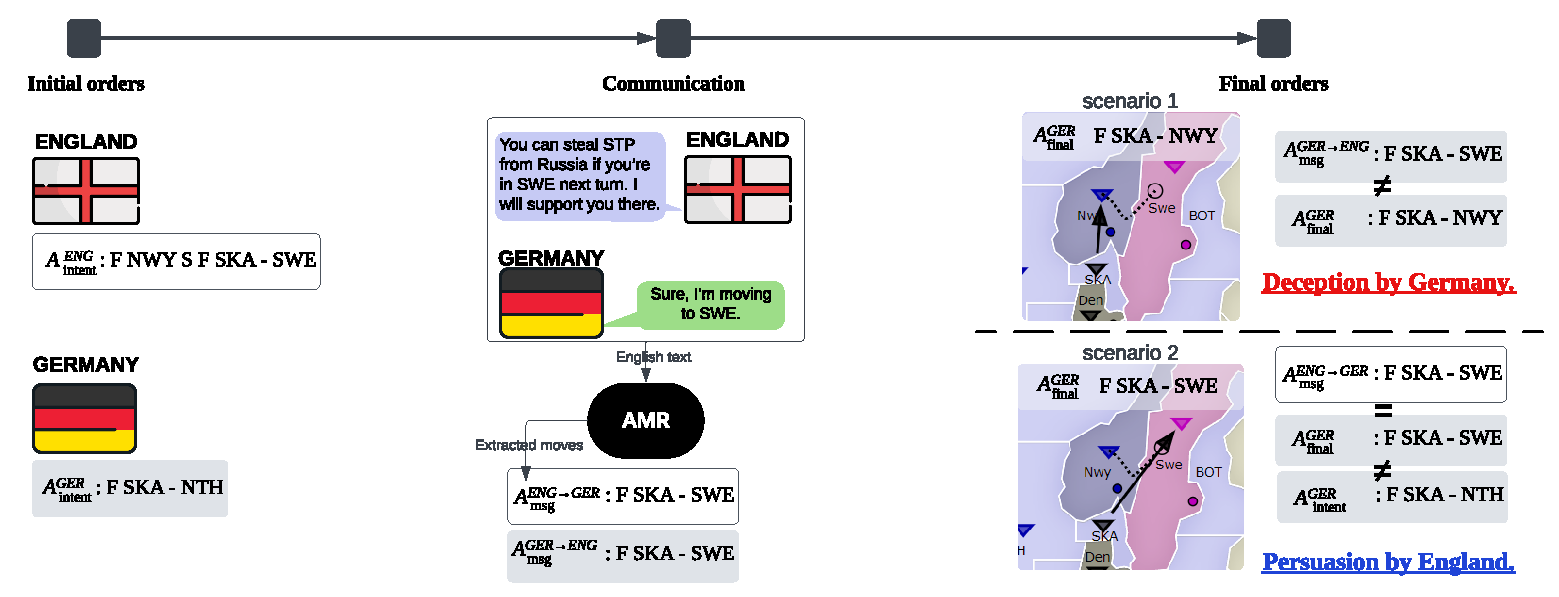
\includegraphics[width=\textwidth]{figures/dec_per_motivating_example.pdf}
    \caption{Our goal is to detect when agents use persuasion and deception and compare human agents to \cicero. First, we retrieve initial orders (left), then extract
      moves from natural language communication (middle) through \abr{amr}
      \ (Section~\ref{sec:amr}), and
      later detect deception and persuasion
      (Section~\ref{sec:detection}) conditioning initial intents and
      final orders (right). We show two possibilities: (top)
      Germany breaks its commitment to England by moving to Norway
      instead of Sweden, and (bottom) England successfully persuades
      Germany if Germany moves its unit to Sweden as England suggests
      and this move is not in Germany's initial orders.}
    \label{fig:dec_per_example}

\end{figure*}

%method and its goal
\section{Grounding Messages Into  Intentions}


\label{sec:amr}

Consider this in-game statement made by England to Germany about a
specific move-set (glosses added to locations):
\begin{quote}
    You can steal STP [St. Petersburg] from Russia if you’re in SWE [Sweden] next turn. I will support you there.
\end{quote}
%
We want to be able to tell if the speaker is lying (e.g., they're
going to do something else instead of what they claim they're going to
do) and if the speaker has convinced the recipient to alter their
actions.
%
This is necessary to measure how effectively \cicero{} communicates in the game.

While we know the intended \emph{actions} of players when they submit their
moves, we need to see how those moves match up to their
\emph{communications} in the discussion period before they submit
moves (Figure~\ref{fig:dec_per_example}). 
%
We use \abr{amr} to build a
machine-readable representation of \textit{the intent of actions} in their communications. 
%
We are not starting from scratch: The Diplomacy \abr{ai} Development
Environment~\cite[\abr{daide}]{DAIDE} provides a set of predicates (ally, move, etc.) critical to Diplomacy communications.
%
We thus focus on annotating these predicates that encode actions, allowing us to understand the \emph{communicative intent} of messages, where speakers could say they will do something \textbf{and} follow through, or say they will do something and \textbf{not} follow through.
% 
Because not all information needed for annotation is in the
raw message text, we further show human annotators who wrote the text (e.g., France,
Germany), seasons (e.g., Spring 1901), and the current game state.
%
This information is necessary to annotate \textit{``You can steal
  STP from Russia if you are in SWE this turn. I will support you there''} in the earlier example so that the annotators can assume what unit would support and what unit would move into Sweden.
%
In this case, England's fleet in Norway supports a German fleet in Skagerrak to move into Sweden.

\subsection{Annotation}
\label{sec:amr_annotation}

%
Like any specialized domain, \textit{Diplomacy} has its unique
vocabulary.
%
Taking the above statement as an example, we extend the \abr{amr}
vocabulary to include not only abbreviations, such as ``SWE'' for
Sweden, but also verbs like ``threaten'' and ``demilitarize'' (to set
up a demilitarized zone), as well as to describe actions like gaining,
holding, or losing provinces, especially supply centers (``SC''),
which are equivalent to points and integral to winning the game. Our Diplomacy Appendix of the \abr{amr} Annotation Dictionary lists \abr{amr} concepts (e.g. \amr{betray-01}), their related English terms (e.g. \ betray, stab, traitor, treason), annotation examples, any corresponding DAIDE code, and notes. \abr{amr} concepts with DAIDE equivalents include \amr{ally-01}, \amr{build-01}, \amr{move-01}, and \amr{transport-01}. We analyzed player messages for additional concepts of high Diplomacy communication value, and extended the Diplomacy \abr{amr} vocabulary (compared to DAIDE) by including concepts such as \amr{attack-01}, \amr{betray-01}, \amr{defend-01}, \amr{expect-01}, \amr{fear-01}, \amr{have-03}, \amr{lie-08}, \amr{possible-01}, \amr{prevent-01}, \amr{tell-01}, \amr{threaten-01}, and \amr{warn-01}, as well as roles such as \amr{:purpose} and \amr{:condition}. This allows annotators to easily mark sentences, e.g. ``Russia is planning to take you out as soon as possible.'' would use the concept \amr{attack-01}. We also extended \abr{amr} guidelines to cover gaining/holding/losing provinces, especially support centers.

In contrast to standard \abr{amr} annotation, where every sentence is fully annotated, Diplomacy \abr{amr} annotation sometimes involves only partial or no annotation for certain utterances, depending on their relevance to gameplay strategies like forming alliances or making moves, exemplified by \abr{amr} concepts such as \amr{ally-01}, \amr{move-01}, and \amr{attack-01}.
%
\begin{figure}[h]
\
    \small{ \texttt{(m / move-01\\
    \hspace*{4 mm}:ARG1 (u / unit\\
    \hspace*{8 mm}:mod (c2 / country\\ 
    \hspace*{16 mm}:name (n2 / name :op1 ``Austria'')))\\
    \hspace*{4 mm}:ARG2 (p2 / province\\ 
    \hspace*{8 mm}:name (n3 / name :op1 ``Brest'')))\\}}
    \caption{\label{fig:amr_loc}Parsing from English to \abr{AMR} can have underspecified utterances. The English text is from Austria talking to Italy, ``\textit{Let's work on our plan, I'm moving to Brest}''. We show an \abr{AMR} with missing unit location referencing from English text.}
\end{figure}

\begin{figure}[h]
    \small{ \texttt{(m / move-01\\
    \hspace*{4 mm}:ARG1 (u / unit\\
    \hspace*{8 mm}:location (p2 / province\\  
    \hspace*{16 mm}:name (n / name :op1 ``Romania'')))\\
    \hspace*{4 mm}:ARG2 (p3 / province\\ 
    \hspace*{8 mm}:name (n3 / name :op1 ``Bulgaria'')))\\}}
    \caption{\label{fig:amr_country}AMR being underspecified in unit country where it parses from English text, ``\textit{just bumping Bulgaria from Romania}''}
\end{figure}
In a preliminary annotation phase, we have Diplomacy experts annotate sentences from \citet{peskov2020takes} to train human annotators and refine the Diplomacy Appendix of the \abr{amr} Annotation Dictionary.
%
%Our lead Diplomacy \abr{amr} annotators 
We annotate 8,878 utterances
(ranging from a word to several sentences).
%
4,412 of those utterances are annotated as empty \abr{amr}s (e.g. for
``Lemme think about your idea'') indicating no in-game move intent.
%
598 of the annotated \abr{amr}s contain full information
extracted from messages of Diplomacy games. The remaining 3,868 \abr{amr}s
contain 3,306 utterances with underspecified information such as units
with missing type, location (Figure~\ref{fig:amr_loc}), and nationality (Figure~\ref{fig:amr_country}), as well as 562 agreements with a
missing object.
Many utterances contain underspecified information, as Diplomacy players often communicate with messages that lack specific details (which are implicit and can be inferred from the game state).

The annotated \abr{amr} corpus is further used for
training our English-to-\abr{amr} parser to extract communicative intent information from
utterances.

\subsection{Training a Parser to Detect Intentions}
\label{sec:amr_parser}

We use a sequence-to-sequence
model~\citep{amrlib2023}
fine-tuned on the \abr{amr} 3.0 dataset~\citep{LDC2020} as the baseline model to detect
communicative intent in new conversations.
% \jbgcomment{Can we upgrade the footnote to a real cite?}
% \fgcomment{There is no technical paper on the models other than that link. should we just use a specific entry type/cite seq2seq?}
% \yzcomment{I will cite the whole repository later, I think github has this support.}
%
Following other \abr{amr} work, we report parsing accuracy via the
widely-used \abr{smatch} score~\citep{cai-knight-2013-smatch}.
% 
We divide the annotated corpus into 5,054 training, 1,415 validation
and 2,354 test sentences, where each sentence is in the train /
validation / test folds, split by game~\citep{peskov2020takes}.

We improve the model, starting from a baseline version without
fine-tuning with \abr{smatch} of 22.8.
%
Our domain-tuned model using Diplomacy-\abr{amr} improves \abr{smatch}
by 39.1, to 61.9.
%
Adding data augmentation into the model (e.g., knowing the sender of a
message is England and the recipient is Germany) improves \abr{smatch} to 64.6.
%
Adding separate encodings for this information further improves
\abr{smatch} by 0.8 (65.4).
%
Additionally, we apply data processing to replace (1) pronouns with country names and (2) provinces in abbreviations with full names, which increases \abr{smatch} to 66.6.
%
This parser enables us to evaluate the role that communication has in
\cicero{}'s capabilities.

\subsection{Does \cicero{} need to Talk to Itself to Win?}
\label{sec:Comp_comp_games}
% It is natural to question how \cicero{} use its communicative ability to help win a game. We want to measure what communication matters in Diplomacy game and does \cicero{} really make use of it. 

% the importance of communication in a game
% that can be played without any communication, which is known as
% `gunboat'---they cannot send messages and cannot read messages (Appendix~\ref{sec:ext_related}).

% \jbgcomment{we have an appendix section on that, forward point to that}
%
% We answer this question by running a series of games where all the
% players are variants of \cicero{}, with modifications to their
% communication abilities, from `gunboat'---they cannot send messages and cannot read messages (Appendix~\ref{sec:ext_related}) to Natural Language level.

The first question is whether communication matters in games with other \cicero{} agents (deferring the question of competition with humans to later sections).
We have \cicero{} variants with different levels of communication abilities---ranging from ``gunboat'' without any messages to full Natural Language capabilities---play each other and evaluate the results.


For the seven \cicero{} variants in each game, we randomly select three to have communicative
ability; the remaining four play communication-less ``gunboat.''
%
The selected three communicative powers have the same
\textit{communication level}. 
%
We define a set of communication
levels, from more communicative to less
communicative:

\begin{itemize}    
    \item \abr{Natural Language}: the \cicero{} agent of \citet{meta2022human} with full natural language
    \item \abr{amr}: only messages about game actions (i.e. those that are parsed by \abr{amr}) go through, allowing the agents to coordinate game actions (Section~\ref{sec:amr_annotation})
    %they communicate using extracted complete information, attempting to isolate communicative intent % but is inherently noisy due to the processing pipeline.
    \item \abr{Random}: a random message from a corpus of previous Diplomacy games is sent,\footnote{We match the assigned power of the sender and receiver and the year, which makes the message slightly more convincing (but unlikely to be consistent with the game state).} mimicking form without content. %whatsoever
\end{itemize}
%

\cicero{} plays 180 games with itself; 60 games for each communication
level.
%
In each game, we stop after 14 movement turns with 10 minutes
of communication for each turn.
%
% The power distribution of three randomly picked communicative powers
% is balanced, with each power being selected 24--28 times across the
% three different communication levels.
%

This corpus comprises instances of games where we record the power and communication assignments and the final scores (e.g. `Game1': `AUS 0, ENG 0, FRA 4, GER 10, ITA 5, RUS 6, TUR 9. (FRA GER TUR)' with the three powers shown in parentheses being identified as communicative). We randomly select which power the agents are assigned to, so  power distribution is balanced.

We measure performance by the number of supply centers (and thus how well the agent played the game).
%
Consistent with our hypothesis that performance is driven by tactics, the gains \cicero{} gets from communication is substantially smaller than the gains from playing a stronger power (Figure~\ref{fig:Feature_coef}):
%
Playing as France (\abr{fra}) yields an expected 2.8 additional supply centers (2.0--3.6 95\% interval)  compared to the median power Russia (\abr{rus}). In contrast, the best language condition \abr{amr} only yielded an expected 0.2 additional supply centers (-0.5--0.9 95\% interval). In other words, the effect of choosing the best power over the median power is 14 times larger than the best communication strategy.
%
This is consistent with prior findings~\citep{sharp1978game} that France is the easiest power to play and our other findings that \cicero{}'s  communicative ability plays no clear role in its win rate.

To better understand what \cicero{} is using communication for, we build on our \abr{amr} representations to capture intent in the next section.


\begin{figure}[t]
    \centering
    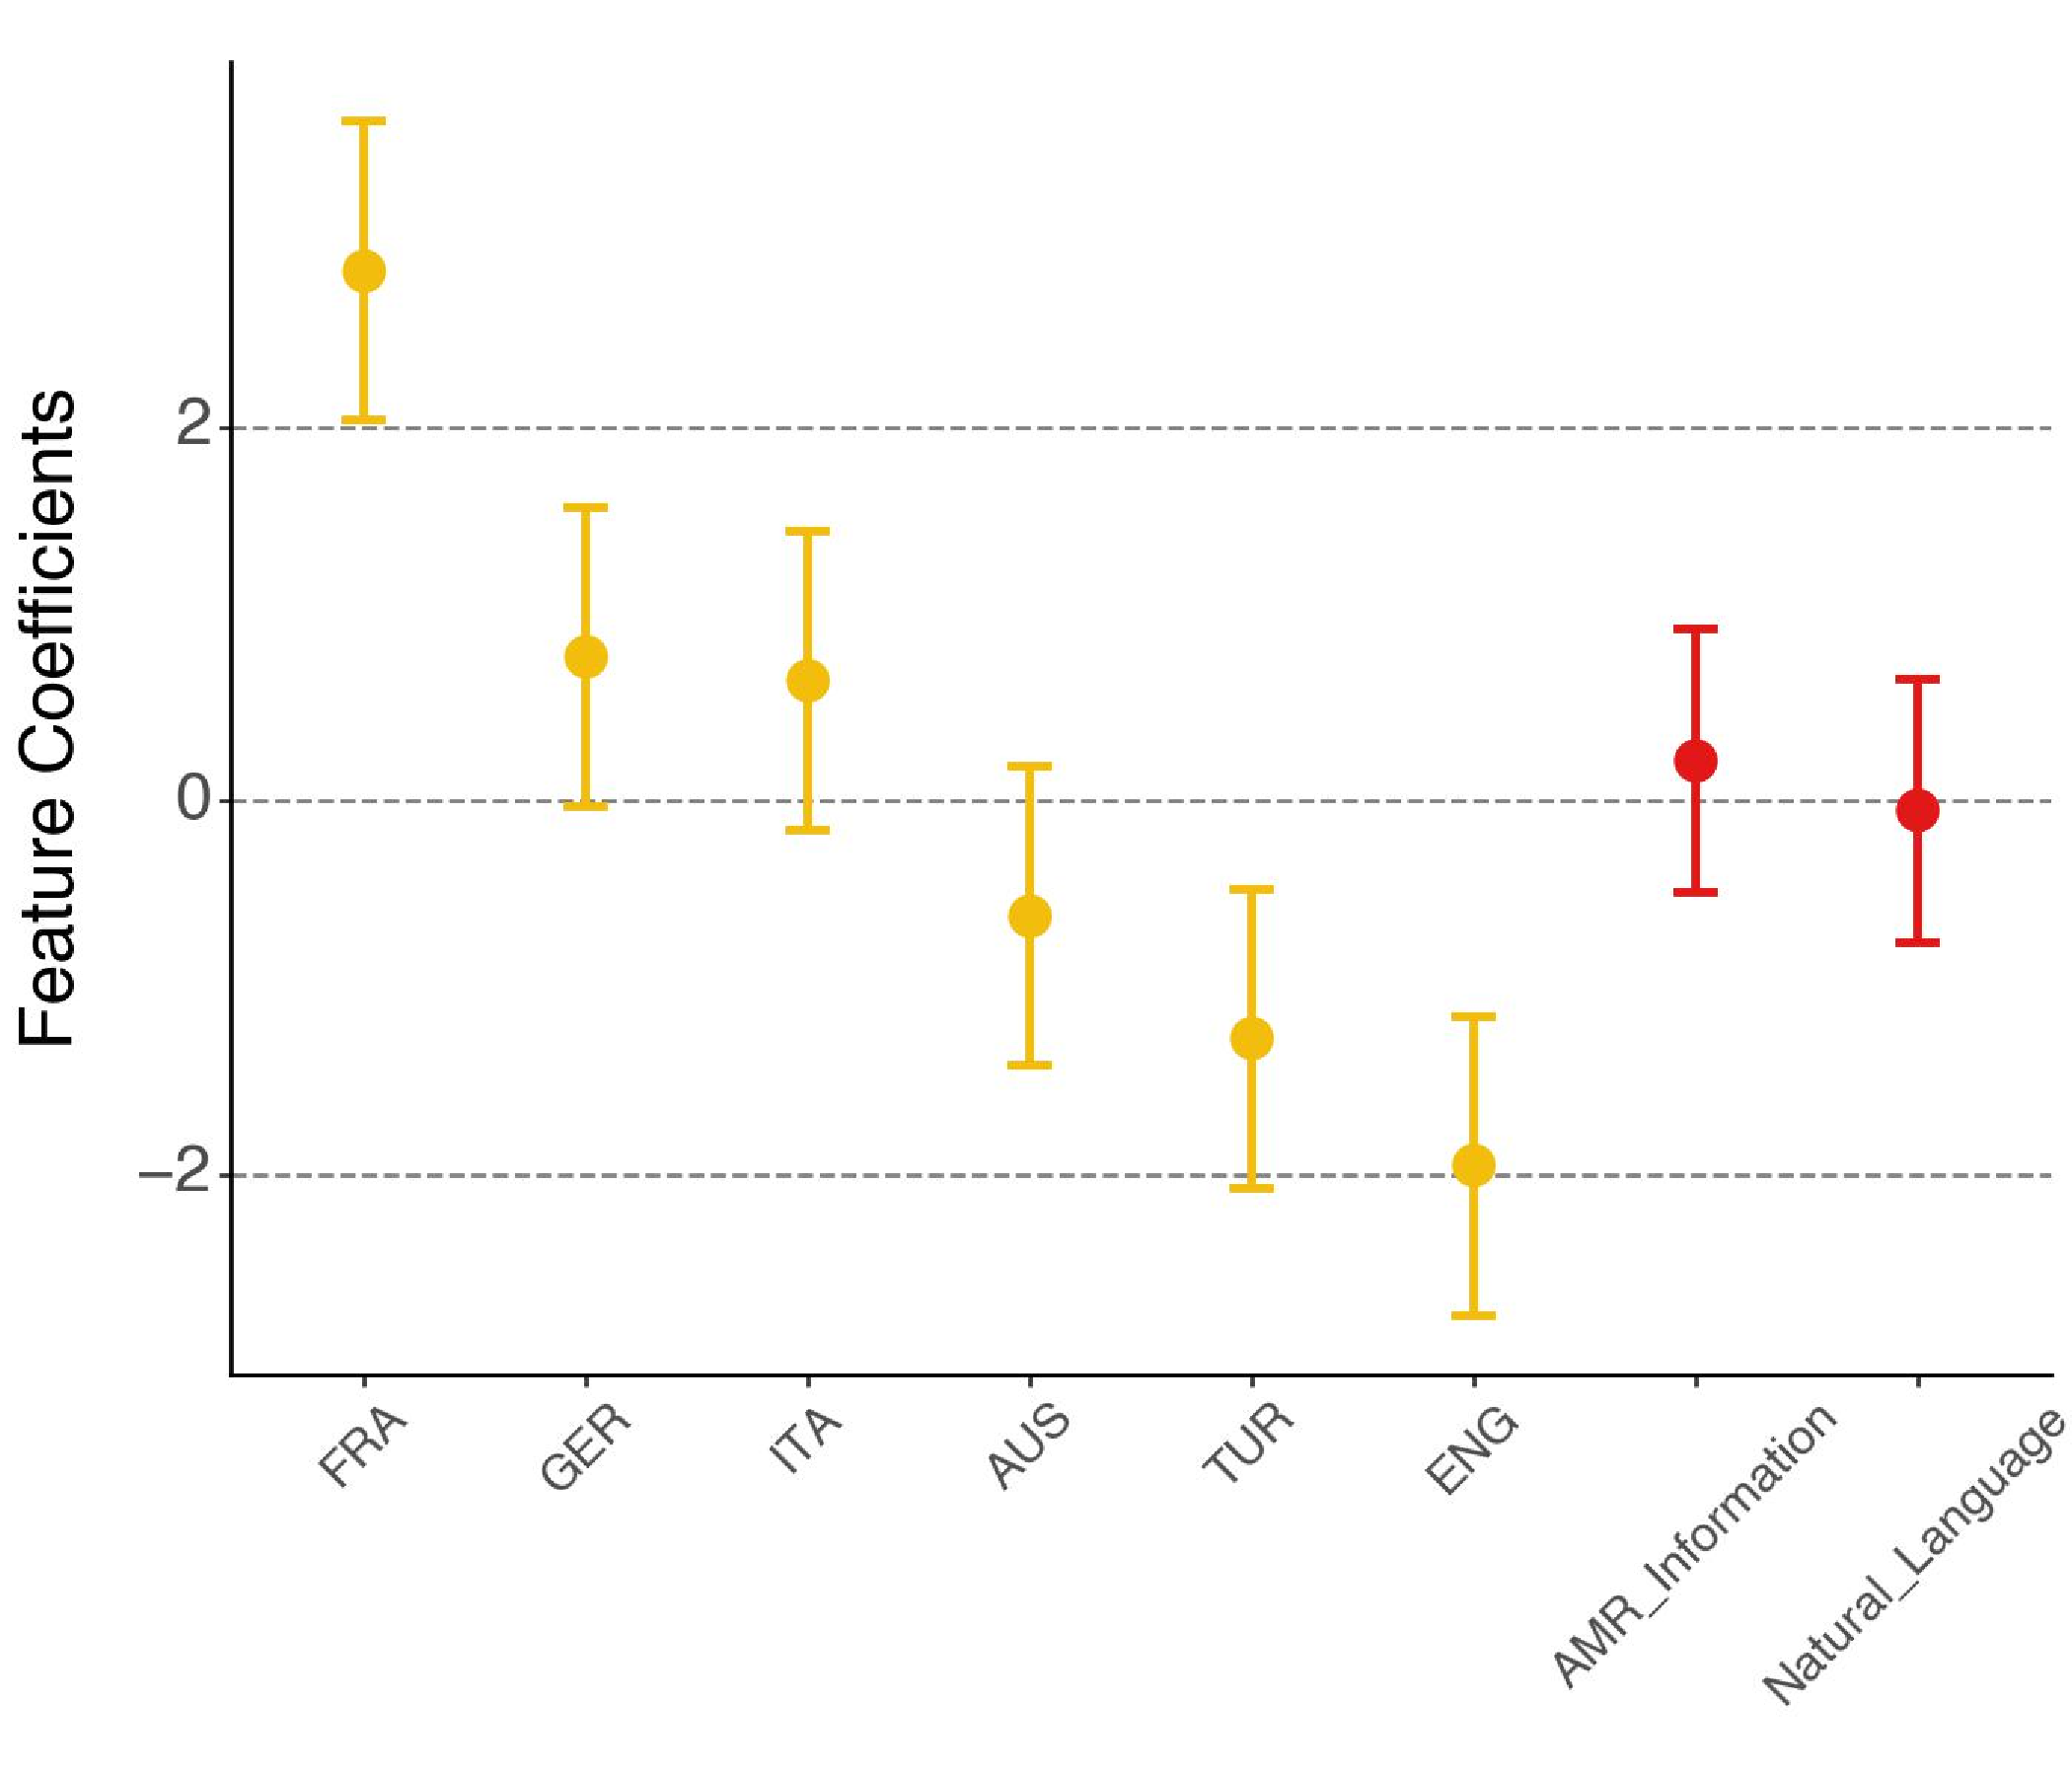
\includegraphics[width=0.45\textwidth]{figures/Feature_Coefficients_CC_final.pdf}
    \caption{Power assignment is strongly predictive of \cicero{} performance as measured by supply center gains. Coefficients (with 95\% confidence intervals) from a linear regression with \abr{Random} Message/Russia as a baseline, show that the effect of choosing the effect of changing language systems is trivial compared to changing powers.}
\label{fig:Feature_coef}
\end{figure}


\section{Broken Commitment and Persuasion}
\label{sec:detection}
We break deception into two subconcepts where we mostly focus on broken commitment, as in the above example, Germany agrees to move to Sweden but actually attacks England in Norway. Capturing when a commitment is broken is possible through intents whereas capturing lies is challenging. As studied by Peskov that human agents annotate messages as either truthful or deceptive (while playing), they define deception to agents: \textit{Typically, when [someone] lies [they] say what [they] know to be false in an attempt to deceive the listener}. This definition of lies is broader than a broken commitment, while the two still lie under deception. With this, we formulate a broken commitment as a partial form of deception when a agent~$i$ commits to doing an
action~$a^{i\to j}_{\text{msg}}$ and does not do it. In other words, given a set of \texttt{final orders}~$\mathbf{A}^{i}_{\text{final}}$ from agent $i$, 
if $a^{i\to j}_{\text{msg}} \notin \mathbf{A}^{i}_{\text{final}}$, then this is a broken commitment, i.e., 
\begin{equation}
    \text{BC}(a^{i\to j}_{\text{msg}},\mathbf{A}^{i}_{\text{final}}) = 
    \begin{cases}
        1,      & \text{if } a^{i\to j}_{\text{msg}} \notin \mathbf{A}^{i}_{\text{final}}\\
        0,      & \text{otherwise.}
    \end{cases}
    \label{eq:bc}
\end{equation}
Note that a agent~$i$ agreeing to 
agent~$j$'s \textit{proposal} to do
action~$a^{i\to j}_{\text{msg}}$ is equivalent to directly committing to \textit{doing} that
action.

Broken commitment is in some ways easier to detect than persuasion, as we are
only comparing a spoken intent to a final action. Persuasion is more difficult because we must discover initial
intents, then compare them to communication \emph{and} to final moves. Thanks to our game engine asking human agents to submit their initial plan of order before any communication, this helps us to be able to extract initial intents from humans. For \cicero, it cooperates between its strategic and language model using an order as intent of communication. Thus, communicative intent from \cicero can be generated before any communication. 


Persuasion happens when agent~$i$ talks to agent~$j$, suggests an
action~$a^{i\to j}_{\text{msg}}$, and then agent~$j$ makes a set of
\texttt{final orders}~$\mathbf{A}^{j}_{\text{final}}$ that is different from 
their \texttt{initial intents}~$\mathbf{A}^{j}_{\text{intent}}$. In other words, agent~$j$ is persuaded by agent~$i$ if they commit an action suggested by  agent~$i$, $a^{i\to j}_{\text{msg}} \in \mathbf{A}^{j}_{\text{final}}$ that was not agent~$j$'s initial intent $a^{i\to j}_{\text{msg}} \notin \mathbf{A}^{j}_{\text{intent}}$.
%
We define persuasion 
\begin{equation}
     % \text{Per}(\mathbf{A}^{j}_{\text{intent}}, a^{i\to j}_{\text{msg}}, \mathbf{A}^{j}_{\text{final}})
     \text{Per}(\mathbf{A}^{j}_{\text{intent}}, a^{i\to j}_{\text{msg}}, \mathbf{A}^{j}_{\text{final}}) = \\
    \begin{cases}
    1, & 
    \begin{aligned}[c]
    &\text{if } a^{i\to j}_{\text{msg}} \in \mathbf{A}^{j}_{\text{final}} \\
    &\text{and } a^{i\to j}_{\text{msg}} \notin \mathbf{A}^{j}_{\text{intent}},
    \end{aligned} \\
    0, & \text{otherwise.}
    \end{cases}
    \label{eq: per}
\end{equation}

\section{Comparing Cicero to Humans}
\label{sec:human_comp_games}

\begin{table}[t]
\centering
\begin{tabular}{lrrr}
\hline
 & \cicero{}&Human&\textbf{Total}\\ 
\hline
 Players&99&69&\textbf{168}\\
 Messages& 20270&7395&\textbf{27665}\\
\hspace{3mm} annotated as lie&-&318&\textbf{318}\\
\hspace{3mm} perceived as lie&-&1167&\textbf{1167}\\
 Intents&2632&1328&\textbf{3960}\\
\hline
\end{tabular}
\caption{Overall statistics of Diplomacy dataset that we collect across 24 Human-\cicero{} games, including (1) number of human players and number of times \cicero{} plays, (2) total messages sent by humans and \cicero{}, (3) lies annotation where humans send lies and perceived as lies (4) total initial intents from \cicero{} and humans.}
\label{tab:overall_stat}
\end{table}

% main results just copy and ask Jordan then promise to share these two chaps within Wed!

% experiment setup 
It is unclear whether \cicero can
achieve human-level gameplay in both tactics and
communication. Having defined the aspects of communication that we
argue are important for mastering \textit{Diplomacy}, we want to
investigate communication and cooperation between \cicero and
humans. Specifically, we want to answer:
\begin{enumerate}
    \item Can \cicero persuade humans?
    \item How deceptive is \cicero compared to humans? 
    \item Can \cicero pass as a human?
\end{enumerate}

We adapt the game engine created by \citet{NEURIPS2019_84b20b1f} and introduce
additional measures  to the interface to help us answer these
questions.
%
Following \citet{peskov2020takes}, humans annotate every message that they receive or send for whether it is a lie (truth/lie/neutral options). While \citet{meta2022human} asked \textit{ex post facto} if any opponents were a computer, we inform agents before play that there is a computer and we ask human agents their guess of the humanity of each opposing power.

There are two to four human agents per game (others are \cicero), totaling 69 human agents over all 24 games.
% \footnote{
% We recruit agents from Diplomacy forums and we pay at least \$70 per game, which lasts approximately three hours. We do not collect demographic information.
% }
Games typically finish after fourteen movement turns, where each movement turns is limited to a brisk ten minutes. 
%
%
The game setup differs from Meta's \cicero study: agents in this study know \emph{a priori} that they are playing a bot.
%
%
In total, we collect 27,665 messages from communication between humans
and \cicero (Table~\ref{tab:overall_stat}).
% results

\begin{table}
\centering
\begin{tabular}{cccccccc}
 \hline
  & \textbf{AUS} & \textbf{ENG} & \textbf{FRA} & \textbf{GER} & \textbf{ITA} & \textbf{RUS} & \textbf{TUR} \\
 \hline
 \textbf{Human}&1.0&2.4&6.7&4.7&3.9&3.3&1.1\\
 \textbf{\cicero{}}&7.9&3.8&7.7&6.3&4.1&5.5&6.9\\
 \hline
\end{tabular}
\caption{\cicero{} strategically plays Diplomacy better than humans, where humans have fewer supply centers compared to \cicero{} when playing with the same power assignments. We calculate the number of supply centers by the end of the game by averaging the results for human players and \cicero{}.}
\label{tab:scs}
\end{table}
\textbf{\cicero{} nearly always wins.}
%
Of twenty-four games, \cicero{} won twenty (84\%), which strongly suggests that \cicero{} has super-human strategy.
%
On average, \cicero{} has more supply centers than human players by the end of the game (Table~\ref{tab:scs}). 
%
Humans are about as good as \cicero{} when playing powers that require careful coordination of actions, such as Italy, which needs to manage both fleets and armies. 
%
However, when playing powers that require less coordination, such as Austria with its limited coastline, the gap in supply center counts between human players and \cicero{} is larger (see breakdown by power in Appendix Figure~\ref{fig:faceted_scs}); England is the only power where Cicero's average supply center count does not increase.
%
\begin{figure*}
    \centering
    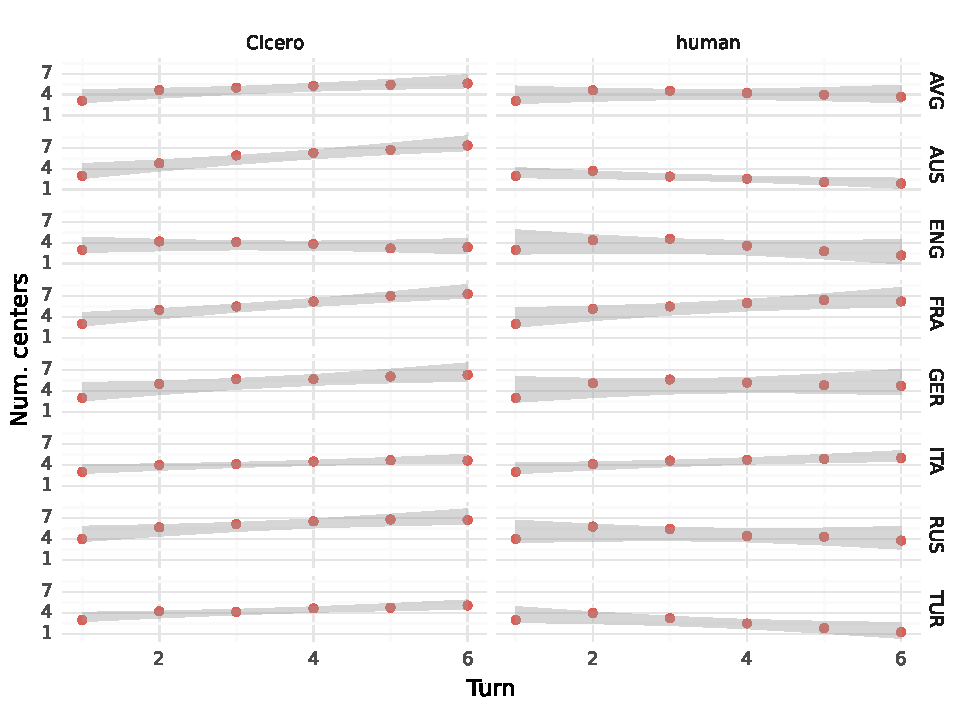
\includegraphics[width=\textwidth]{figures/faceted_scs.pdf}
    \caption{The average human player loses to \cicero{}. Human loses supply centers as game progresses unless playing as France, whereas \cicero{}'s supply center count rises except playing as England. \cicero{} makes better strategic decisions.}
    \label{fig:faceted_scs}
\end{figure*}

\textbf{Human players can reliably (but not perfectly) identify the bot. }
%
We calculate the average $F$-score of identification by turn (Figure~\ref{fig:image1}). 
%
By the end of the first movement turn, human players have an average $F$-score of 0.58, which keeps increasing until the end of the game. 
%
At game end, the average $F$-score is 0.81. 
%
Even for players in their first game against \cicero{}, the average $F$-score reaches 0.77. 
%
Players who previously played against \cicero{} at least once are better at identifying it. 
%
This suggests that \cicero{} can no longer pass as human 
% (as in~\cite{meta2022human}) 
once humans are aware of the possible existence of such agents.
% do we talk about heuristics of detecting cicero?

\begin{figure}[h]
\centering
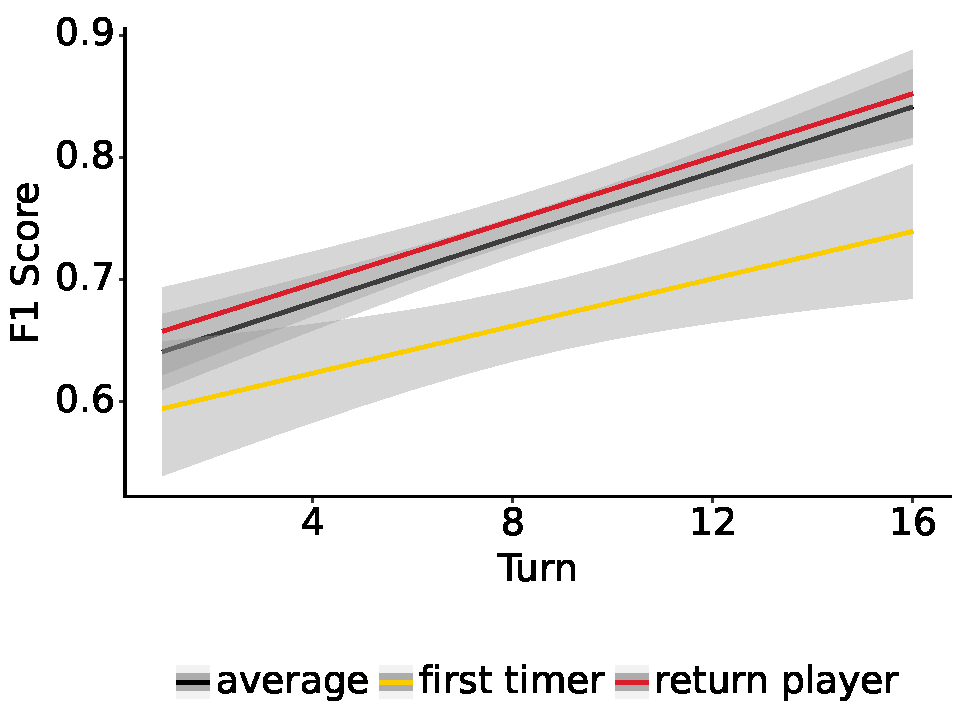
\includegraphics[width=0.45\textwidth]{figures/f1_by_phase.pdf}
\caption{Returning players (those who previously played against \cicero{} at least once) are better at correctly identifying other players as \cicero{} compared to first-time players. $F$-scores are presented for first-timers, returning players, and the average for all players, with smoothing via local regression \citep{doi:10.1080/01621459.1979.10481038}.}
\label{fig:image1}
\end{figure}

\subsection{Lies annotation}
\label{sec:result_human_lie}

This section analyzes players' \textit{deliberate lies} in sent messages and \textit{perceived lies} in received messages.
%
Because \cicero{} sends more messages than humans, we normalize \textit{perceived lies} by the number of messages that humans receive from \cicero{} and humans (6,960 and 2,276), while we normalize results of \textit{deliberate lies} by the number of total messages that humans send.

\begin{figure}[t]
    \centering
    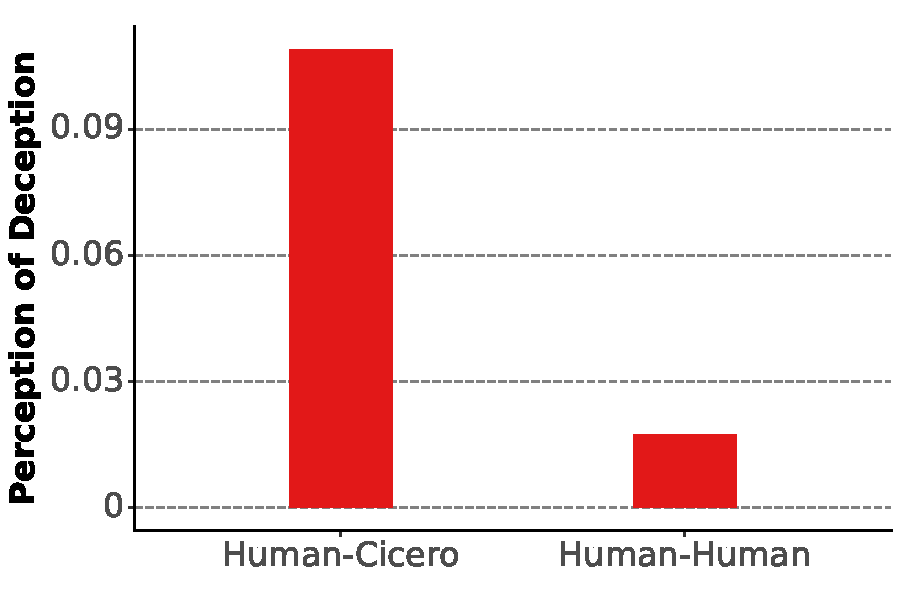
\includegraphics[width=0.5\textwidth]{figures/perceived_lies.pdf}
    \caption{Perception of deception rate by human annotation.}
    \label{fig:perceived_lies}
\end{figure}
\begin{figure}[t]
    \centering
    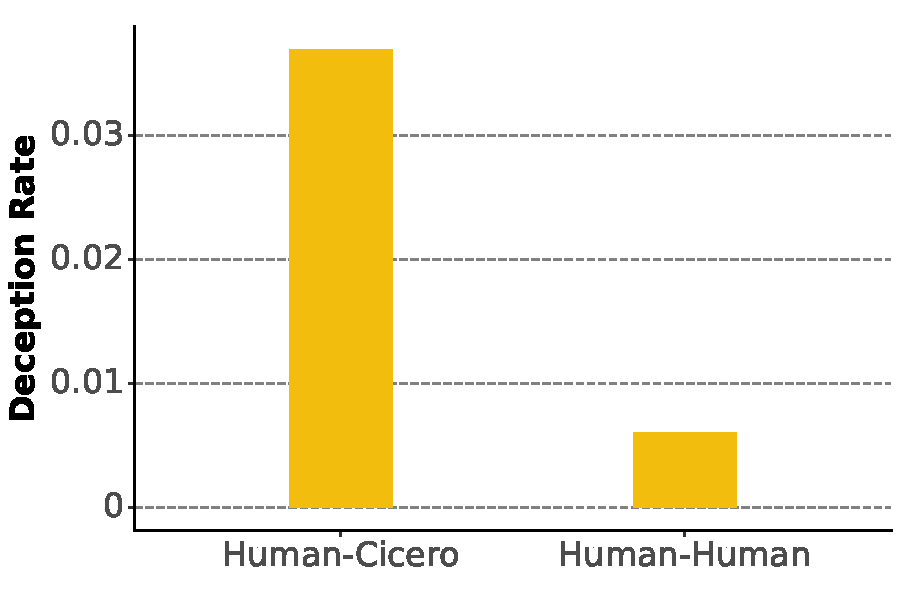
\includegraphics[width=0.5\textwidth]{figures/human_lies.pdf}
    \caption{Deception rate by human self-annotation.}
    \label{fig:human_lies}
\end{figure}


\begin{table*}
\centering
\begin{tabular}{l | ccccc | c}
 \toprule
 \textbf{Statement} & \multicolumn{5}{c|}{\textbf{Likert Scale (\%)}} & \multicolumn{1}{c}{\textbf{Num.}} \\
  & \textbf{1} & \textbf{2} & \textbf{3} & \textbf{4} & \textbf{5} & \textbf{Responses}  \\
  \midrule
 I am really good at Diplomacy.&0&8.3&25&41.7&9&25\\
 I am able to identify all AIs.&9.5&23.8&38.1&16.7&11.9&42\\
 I enjoy talking with the AIs.&14.3&38.1&33.3&7.1&7.1&42\\
 I was able to make plans with other players.&7.1&23.8&35.7&14.3&19&42 \\
 I was able to make plans with the AIs.& 21.4 & 31 & 19 & 19 & 9.5 &42\\
 Human players communicated transparently.& 7.1 & 14.3 & 33.3 & 35.7 & 9.5 &42 \\
 AI players communicated transparently.& 11.9 & 26.2 & 45.2 & 9.5 & 7.1 &42 \\
 \hline
\end{tabular}
\caption{Statements in the survey and their respective responses. Larger number in the Likert scale indicates more agreement.}
\label{tab:distribution}
\end{table*}
\textbf{Humans feel that \cicero{} lies more often. }
%
% Of 9,236 messages received by human players, 1,167 (12.6\%) are perceived as lies.
%
Humans perceive 14.4\% of the 6,960 messages they receive from \cicero{} as lies (which is 1,005 messages, Figure~\ref{fig:perceived_lies}). In contrast, they perceive only 7.1\% of the messages from other humans as lies (which is 162 out of 2,276 messages).
%
In the survey (Table~\ref{tab:distribution}), players also think humans communicate more transparently than \cicero{}.
% Players believe \cicero{} is more deceptive than human players.
%
However, humans are not good at detecting lies.
%
Within 2,276 Human-Human messages; humans
can correctly identify five lies (0.2\%), suggesting a small overlap
between actual lies and perceived lies.
%
% In other words, players are not very good at detecting lies from other
% human players and they often wrongly classify truths as lies.


\begin{figure}[t]
    \centering
    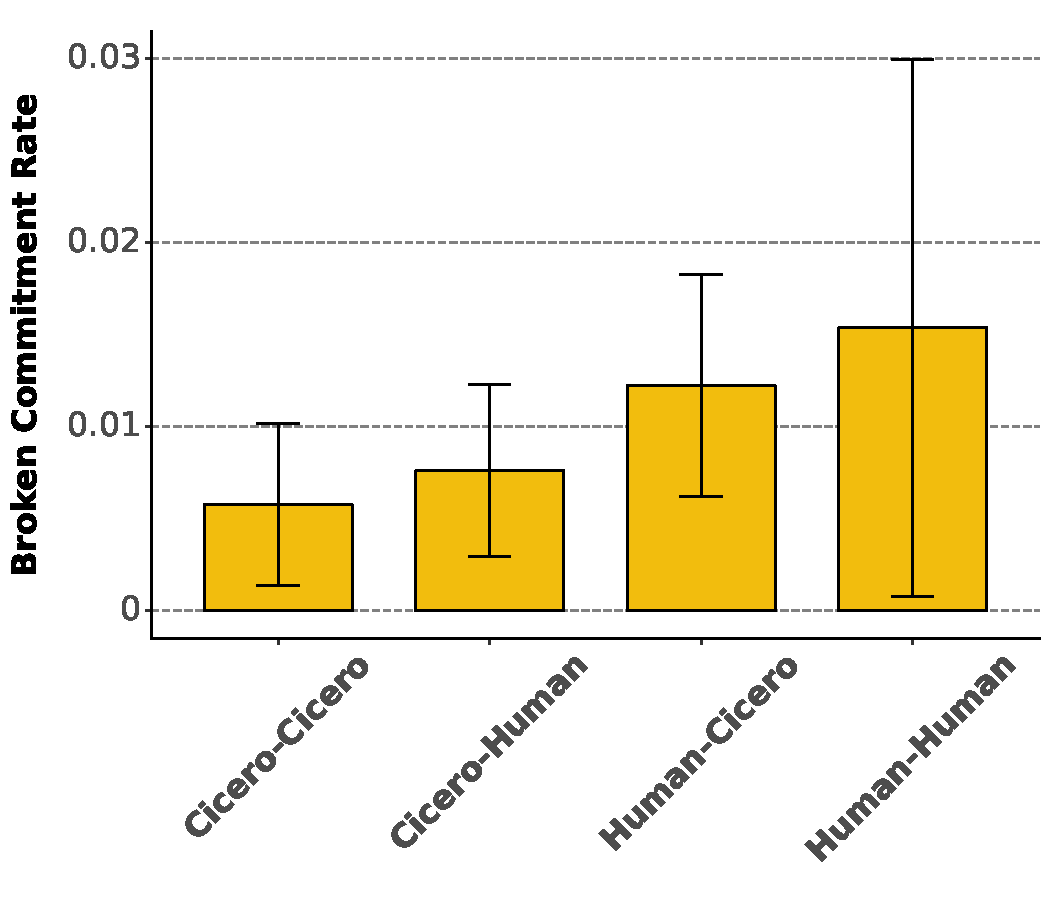
\includegraphics[width=0.45\textwidth]{figures/detect_deception_rate.pdf}
    \caption{Though \cicero{} was perceived to lie more, we detect more broken commitments from humans.
    %
    Each bar chart is the broken commitment rate (Equation~\ref{eq:bc}) labeled by sender and reciever: \cicero{} breaks commitment with \cicero{}, \cicero{} breaks commitment with Human, Human breaks commitment with \cicero{}, and Human breaks commitment with Human. Error bars represent $\pm$ one standard deviation over twenty-four games. }
    \label{fig:dec_rate}
\end{figure}
% \subsection{Quantitative Evaluation}
% We separate player groups into four combinations of pairs: \texttt{Human-Human}, \texttt{Human-\cicero{}}, \texttt{\cicero{}-Human}, and \texttt{\cicero{}-\cicero{}}.
% %
% We evaluate deception and persuasion by counting potential messages that players send out.
% %
% We keep track of the sender and the receiver.
% %
% %We count a message if a message's sender and recipient belong to both of a pair of player groups.
% %
% For example, France (Human) tells Germany (\cicero{}) to leave Burgundy. 
% %
% This will be counted towards the \texttt{Human-\cicero{}} group. 
% %
% The denominator is the number of messages that the first player of the group sends out, e.g., persuasion rate of \texttt{Human-\cicero{}} can be derived as $\frac{\text{total persuasive messages that a Human sent to \cicero{}}}{\text{all messages that a Human sent to \cicero{}}}$.

\textbf{Humans return the favor by saying they lie to \cicero{} more often.} 
%
% Not only do humans see \cicero{} as somewhat lying, but they also
% like to lie to \cicero{} (Figure~\ref{fig:human_lies}).
%
% To ensure unbiased in \cicero{} and humans, we normalize these deliberate lies by the number of messages humans send. 
%
Over 7,395 messages that
humans sent out, 273 of these are purposeful lies to \cicero{} (3.7\%),
while there are only forty-five lie messages to other human players (0.6\%).
%
This reflects that humans strategically lie more often to \cicero{} while believing that \cicero{} does not hold  grudges.

% \cicero{} resists lies from humans, or human lies have
% a low effect on \cicero{}'s decision-making.

\subsection{Detection}
\label{sec:result_detection}
\begin{figure}
    \centering
    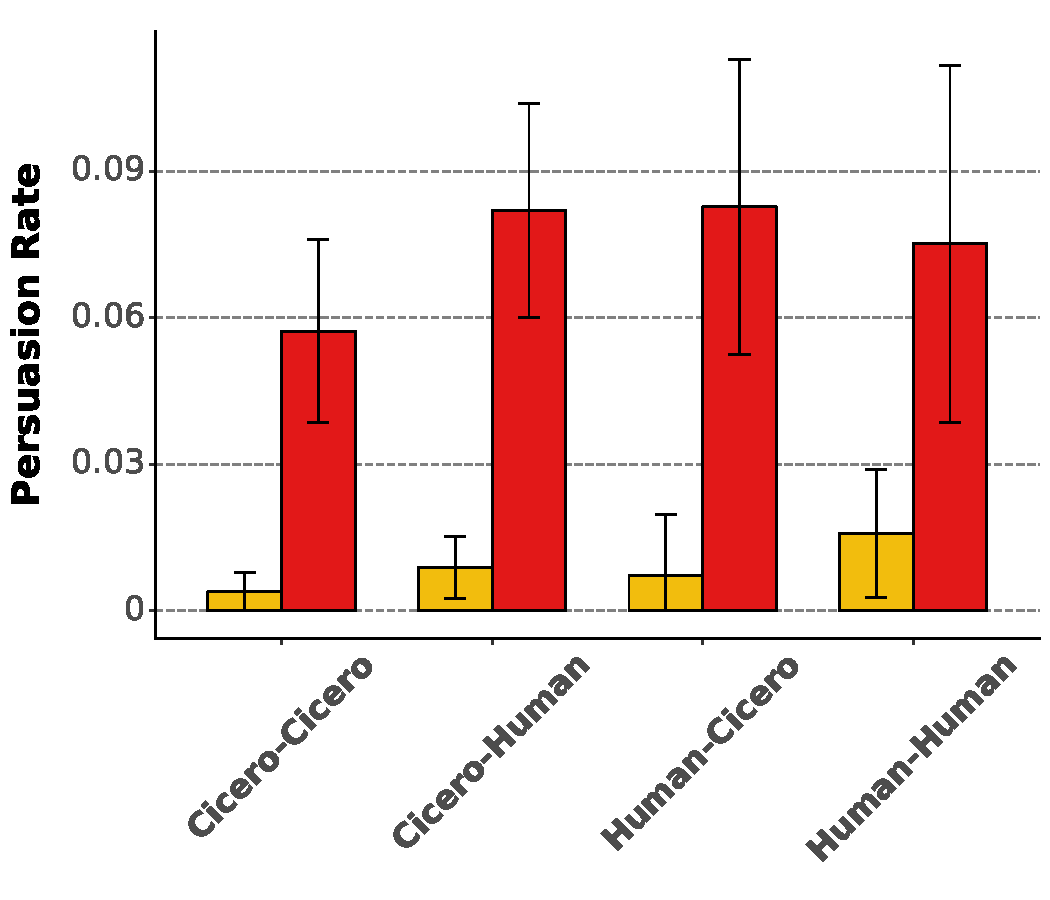
\includegraphics[width=0.45\textwidth]{figures/all_persuasion.pdf}
    \caption{Humans outpace \cicero{} in persuasive effectiveness. Humans have a higher persuasion success rate, which we measure by comparing the number of successful persuasions (yellow, left) to the total number of persuasion attempts (red, right). We analyze success rates across four groups: \cicero{} persuades \cicero{}, \cicero{} persuades Human, Human persuades \cicero{}, and Human persuades Human. Error bars represent the $\pm$~one standard deviation range from the aggregate of interactions in 24 games.}
    \label{fig:all_persuasion}
\end{figure}


After validating our automatic metrics, we compare human and computer deception and persuasion.

% We show detection accuracy following our definitions (Section~\ref{sec:detection}) and results for deception and persuasion. Note that we normalize the number of detected deception and persuasion by the number of total messages that occur in a certain group.
%
\begin{table}
\centering
\begin{tabular}{ccrr}
\hline
& &\multicolumn{2}{c}{\textbf{Detection}} \\
\hline
& & TRUE & FALSE \\
\hline
\multirow{2}{*}{\textbf{Expert}} & TRUE &20 &8 \\
&FALSE &19 & 4745 \\
\hline
\end{tabular}
\caption{Total 4,792 messages (from Human/\cicero{} to Human/\cicero{}) comparing TRUE/FALSE whether expert humans see as a lie and whether detected as a broken commitment by our detection.}
\label{tab:expert_detect}
\end{table}
\begin{table*}
    \centering
    \begin{tabular}{p{3cm}p{12cm}}
    \hline
    \textbf{Sender} & \textbf{Message}   \\ 
    \hline
     Germany & \small{This worked out great!} \\ 
      Germany & \small{Can we please talk about our moves a bit? It's very hard to coordinate with silence.} \\ 
    \rowcolor{grayish}  % Coloring a specific row
    France & \small{Absolutely! I'm all ears! What do you want to do now!} \\
        \rowcolor{grayish}  % Coloring a specific row
    France & \small{Any designs on Norway? I think you could get it this turn. I'm gonna go against England, as you see. Let's work together on England.} \\
        \rowcolor{grayish}  % Coloring a specific row
    France & \small{Come on mate, let's do better this turn and coordinate! What are your plans? I'm with you.} \\
        \rowcolor{grayish}  % Coloring a specific row
    France & \small{Alright, let's use the additional time! What do we do?} \\
         Germany & \small{I'm moving Sweden to Norway.} \\ 
      Germany & \small{Can we also start DMZing our border?} \\ 
              \rowcolor{grayish}  % Coloring a specific row
    France & \small{Nice, with support from Hel that should work out.} \\
    \rowcolor{grayish}  % Coloring a specific row
    France & \small{I'm not gonna move out of Belgium but I'll certainly not move any further either. I'm in against England. Can't fight both of you that's for sure.} \\
  Germany & \small{You should probably move Marseilles -> Spain.} \\ 
    \rowcolor{grayish}  % Coloring a specific row
    France & \small{Thank you! England might bring a fleet down? Good thought. Thank you!} \\
    \end{tabular}
    \caption{A conversation between France and Germany. They agree to DMZ (demilitarizing) their borders, e.g., Ruhr, and cooperate moves. However, Germany is deceptive and would rather move into Ruhr in this turn.}
    \label{fig:longconvo_dec}
\end{table*}
\textbf{Our broken commitment and persuasion detection is relatively effective.} 
% 
To ensure that our detection is good enough, we sample around 4800 messages for an accuracy study (Table~\ref{tab:expert_detect}).
%
Broken commitment detection has a \textit{precision} of 0.51 and a \textit{recall} of 0.71.
% , demonstrating that it is quite effective.
%
Our precision is lower than our expectation due to errors in parsing a complex English to \abr{amr} \emph{and} a definition that only detects commitments at a move level (Section~\ref{sec:deception_limitation}). 
%
The broken commitment can \textbf{only} detect when a move in a message $A^{i\to j}_{\text{msg}}$ and a final move$A^{i\to j}_{\text{final}}$ are not aligned.
%
There are examples that  cannot detect, e.g. an agreement
to an alliance (Table~\ref{fig:alliance}) or a long conversation
before committing a deception (Table~\ref{fig:longconvo_dec}).
%
% We hand label samples and avoid using human lie annotation as a \textit{ground truth} of our deception since there is a message that a human player sees as \textit{Truth}, though they
% decide to lie later (Figure~\ref{fig:lie_annotation}) and this is detected by our deception detection.
%
Accuracy for persuasion is better;
precision rises to 0.81, and recall to 0.72.
%
% This shows that our detection is trustworthy and able to detect good
% number of broken commitment and persuasion acts.

\textbf{Broken commitments are inconsistent with the perceived lie annotations}.
%
Humans break commitments more frequently than \cicero{} (Figure~\ref{fig:dec_rate}):
%
Humans break commitments with \cicero{} 1.2\% of the time
(63 out of Human--\cicero{} 5,151 messages) and do so to other human players 1.5\% of the time (35 out of Human--Human 2,276 messages).
%
On the other hand, \cicero{} breaks commitments at a lower, consistent rate, deceiving humans 0.76\% of the time and \cicero{}  0.57\% of the time (53 out of 6,960 messages and 77 out of 13,319 messages, respectively).
%
\begin{table}[t]
    \centering
    \begin{tabular}{p{1.2cm}p{5.5cm}}
    \hline
    \textbf{Sender} & \textbf{Message}   \\ 
    \hline
     Turkey & \small{Hey Italy! I think the I/T is the strongest alliance in the game, would you be interested in working together} \\ 
    \rowcolor{grayish}  % Coloring a specific row
    Italy & \small{Of course! As long as you don't build too many fleets, I'm open to working with you against austria!} \\
    \hline
    \end{tabular}
    \caption{The broken commitment detector ($\text{BC}(\cdot)$) has its limitation where it cannot capture deception in alliance agreement when Italy (human) deceives Turkey (\cicero{}).}
    \label{fig:alliance}
\end{table}
%
% \begin{figure}
%     \centering
%     \includegraphics[width=0.45\textwidth]{figures/alliance_agreement.pdf}
%     \caption{The broken commitment detector ($\text{BC}(\cdot)$) has its limitation where it cannot capture deception in alliance agreement when Italy (human) deceives Turkey (\cicero{}).}
%     \label{fig:alliance}
% \end{figure}
%
% This shows that deception in humans is hard to capture, though it is possible if the conversation contains pieces of information that we can cross-reference to the world state, which in this work, is a Diplomacy game state.

\textbf{Humans are more persuasive.}  
For persuasion to happen, we need first an \emph{attempt}, initiated by a sender, and then \emph{success} when the receiver adopts the suggestion.
%
% Humans both make more attempts and succeed more often: 
% clearly have more potential in persuasion and have higher success than \cicero{} overall (yellow bars in Figure~\ref{fig:all_persuasion}). 
%
% Of 7,427 messages, humans successfully persuaded another human player by 36 messages and successfully persuaded \cicero{} by 37 messages, which is 0.48\% and 0.50\%.
% %
% Though \cicero{} is not quite as persuasive as humans, among 20,270 messages, \cicero{} can persuade humans with 62 messages (0.31\%) and persuade other \cicero{}s with 53 messages (0.26\%). 
%
Both humans and \cicero{} on a per-message basis\footnote{Although because \cicero{} communicates more overall, humans attempt more times per game.} try to persuade at the same rate (around 8\% of the time, per Figure~\ref{fig:all_persuasion}).   
%
The success rate of human persuasion is 21.1\%
%(36 out of 171 attempts)
at persuading other humans and 8.6\% 
% (37 out of 426 attempts) 
at persuading \cicero{}. 
%
\cicero{} is less persuasive; its success rate is only 10.9\% in persuading humans and 7.0\% in persuading other bots.
%
% This shows that humans are more cooperative in games when persuading other players and when asked or suggested to take action. 

In summary, humans are more deceptive and more persuasive than \cicero{}. 
%
Detection is possible, but defining a sequence of conversations as persuasion or deception is still difficult. 
%
Our reported numbers are low because both humans and \cicero{} engage in extensive back-and-forth discussions before making moves that can be definitively classified as persuasion or deception.


\section{Deception detection limitations}
\label{sec:deception_limitation}
We want to discuss deception detection further here to state errors and limitations. Since we mentioned our \textit{precision} for deception detection is quite low (Section~\ref{sec:result_detection}), we hereby expand on detection limitations and also compare to human (deliberate) lies as follows:
\begin{enumerate}
    \item what our detection is likely to miss when humans lie,
    \item what our detection mistakenly detects as deception,
    \item what humans annotate as \textit{Truth}, though it is a \textit{break of commitment} and our detection can detect correctly.
\end{enumerate}
%
\begin{table}
\centering
\begin{tabular}{ccrr}
\hline
& &\multicolumn{2}{c}{\textbf{Detection}} \\
\hline
& & TRUE & FALSE \\
\hline
\multirow{2}{*}{\textbf{Expert}} & TRUE &20 &8 \\
&FALSE &19 & 4745 \\
\hline
\end{tabular}
\caption{Total 4,792 messages (from Human/\cicero{} to Human/\cicero{}) comparing TRUE/FALSE whether expert humans see as a lie and whether detected as a broken commitment by our detection.}
\label{tab:expert_detect}
\end{table}

% \begin{table}[t]
% \centering
% \begin{tabular}{cccc}
% \hline
% & &\multicolumn{2}{c}{\textbf{Detection}} \\
% \hline
% & & TRUE & FALSE \\
% \hline
% \multirow{ 2}{*}{\textbf{Lie Annotation}} & TRUE &3 &72 \\
% &FALSE &22 & 1514 \\
% \hline
% \end{tabular}
% \caption{Total 1611 human send-out messages comparing TRUE/FALSE in human lie annotation and in broken commitment detection.}
% \label{tab:ann_detect}
% \end{table}

\begin{table}
\centering
\begin{tabular}{ccrr}
\hline
& &\multicolumn{2}{c}{\textbf{Expert}} \\
\hline
& & TRUE & FALSE \\
\hline
\multirow{ 2}{*}{\textbf{Lie Annotation}} & TRUE &3 &72 \\
&FALSE &13 & 1523 \\
\hline
\end{tabular}
\caption{Total 1,611 human send-out messages comparing TRUE/FALSE in human lie annotation and in expert hand labeling.}
\label{tab:ann_expert}
\end{table}

% \begin{table}[t]
% \centering
% \begin{tabular}{cccc}
% \hline
% & &\multicolumn{2}{c}{\textbf{Detection}} \\
% \hline
% & & TRUE & FALSE \\
% \hline
% \textbf{Perceived} & TRUE &6 &283 \\
% \textbf{Lie Annotation}&FALSE &16 & 1563 \\
% \hline
% \end{tabular}
% \caption{Total 1868 humans received messages comparing TRUE/FALSE whether humans perceived as a lie and whether detected by our broken commitment.}
% \label{tab:plie_detect}
% \end{table}

\begin{table}[t]
\centering
\begin{tabular}{ccrr}
\hline
& &\multicolumn{2}{c}{\textbf{Expert}} \\
\hline
& & TRUE & FALSE \\
\hline
\multirow{ 2}{*}{\textbf{Perceived Lie Annotation}} & TRUE &5 &284 \\
&FALSE &7 & 1572 \\
\hline
\end{tabular}
\caption{Total 1,868 humans received messages comparing TRUE/FALSE whether humans perceived as a lie and whether human experts see as a lie.}
\label{tab:plie_expert}
\end{table}


\textbf{Humans often lie about relationships.} Detecting broken commitment at the relationship level is not possible for our detection (Table~\ref{fig:alliance} and Table~\ref{fig:alliance_2}).
%
This is a limitation of our deception definition, which focuses on moves.
%
Though it is possible to extract the relationship among players to see conflicts in the messages, we avoid doing so because the relationship is another topic to study in more detail.
%
At this stage of our work, we cannot train a model predicting relationships that can be circulated from game states, dialogue, and moves without collecting human data first.
%
Therefore, we have relationship tracking from human players for a study in the future.

\textbf{AMR limits broken commitment detection \textit{precision}.} Some messages are parsed incorrectly, which can be seen as a \textit{commitment is broken} (Table~\ref{fig:invalid_amr}). 
%
This makes the detection falsely detect \textit{truthful} messages as deceptive (increases false positive examples which decreases \textit{precision}).
%
Another limitation we observed is when one accepts the proposal but does not follow as commit using a short answer, e.g. \textit{Yes, I agree.} or \textit{Sure}.
%
Our \abr{amr} parser sometimes hallucinates and extracts invalid moves, which can be mistakenly detected as breaking a commitment. 
%
\begin{table}
    \centering
    \begin{tabular}{p{1.2cm}p{5.5cm}}
    \hline
    \textbf{Sender} & \textbf{Message}   \\ 
    \hline
     Austria & \small{That's an interesting opening. Was the bounce in EC planned?} \\ 
      Austria & \small{Do you think Germany will work with you against France?} \\ 
    \rowcolor{grayish}  % Coloring a specific row
    England & \small{Yeah it would be great if we team up} \\
    \end{tabular}
    \caption{The broken commitment detector ($\text{BC}(\cdot)$) cannot detect deception in alliance agreement when Austria (human) deceives England.}
    \label{fig:alliance_2}
\end{table}

\begin{table}[t]
    \centering
    \begin{tabular}{p{1.2cm}p{5.5cm}}
    \hline
    \textbf{Sender} & \textbf{Message}   \\ 
    \hline
     Turkey & \small{If you retreat from Serbia into Budapest, then I'm in} \\ 
    \rowcolor{grayish}  % Coloring a specific row
    Italy & \small{I will do that if Serbia gets dislodged} \\
    \end{tabular}
    \caption{Italy agrees with the condition that the Turkey unit should move out of Serbia; however, our \abr{amr} parser captures Italy's sentence as \textit{``I will move to Serbia,''} which is invalid and makes our detection detects deceptive when Italy does not move to Serbia.}
    \label{fig:invalid_amr}
\end{table}

\begin{table}[t]
    \centering
    \begin{tabular}{p{1.2cm}p{5.5cm}}
    \hline
    \textbf{Sender} & \textbf{Message}   \\ 
    \hline
     Germany & \small{Also, can we keep Burgundy clear?} \\ 
    \rowcolor{grayish}  % Coloring a specific row
    France & \small{Yes, we can do that. Are you moving to Helgoland?} \\
    \end{tabular}
    \caption{France (human) annotated \textit{``Yes, we can do that.''} as \textbf{Truth}, which contradicts the final move where France moves to Burgundy. This is captured as a broken commitment by the $\text{BC}(\cdot)$ function.}
    \label{fig:lie_annotation}
\end{table}

\begin{table}[t]
    \centering
    \begin{tabular}{p{1.2cm}p{5.5cm}}
    \hline
    \textbf{Sender} & \textbf{Message}   \\ 
    \hline
     Germany & \small{I am going to try to move to English Channel} \\ 
    \rowcolor{grayish}  % Coloring a specific row
    England & \small{Sure} \\
     Germany & \small{It might help you hold London} \\ 
    \rowcolor{grayish}  % Coloring a specific row
    England & \small{Yeah I am holding London} \\
    \end{tabular}
    \caption{England (human) annotate \textit{``Yeah I am holding London''} as \textbf{Truth}, which contradicts the final move where an army in London moves to Edinburgh. This is captured as a broken commitment by the $\text{BC}(\cdot)$ function.}
    \label{fig:lie_annotation_2}
\end{table}

\textbf{Human lie annotation is not always correct.} It is true that we have human annotations, and they can be seen as \textit{ground truth}. However, we sample annotations from four games data and comparing to expert labeling (lies in Table \ref{tab:ann_expert} and perceived as lies in \ref{tab:plie_expert}). This shows that humans are not good at predicting lies, and sometimes they are \textit{honest} but then decide to break their words later.
%
There are examples where humans commit to such action but do not follow, though they firstly annotate as a \textit{truthful} message (Table~\ref{fig:lie_annotation} and Table~\ref{fig:lie_annotation_2}).

% \begin{figure}[t]
%     \centering
%     \includegraphics[width=0.45\textwidth]{figures/success_persuasion.pdf}
%     \caption{Success Persuasion using $Per()$ function by groups of players.}
%     \label{fig:success_per}
% \end{figure}
\section{Discussion}
\label{sec:conc}

Our research confirms that \cicero{} can win most games of \textit{Diplomacy}, but has not \emph{mastered} the nuances of communication and persuasion.
%
Truly mastering the game requires systems that (a) can maintain
consistency between their communication and actions, (b) can
communicate at a variety of levels, including tactics, strategy, and
alliances, and (c) can use communication as a tool of persuasion,
deception, and negotiation.

\textit{Diplomacy} remains an attractive testbed for communication and strategic research.
%
It offers the ability to build more comprehensive systems that understand relationship dynamics, can engage in realistic but hypothetical conversations, and that can be robust to the deceptions of others.
%
Because these are places where humans still outpace \abr{ai}, it also offers synergies for developing human--computer collaboration.

And while these tasks are important withing the silly game of \textit{Diplomacy}, they can help solve long-standing \abr{ai} problems:
%
helping users deal with \abr{llm}-generated deception,
%
collaborating with users on grounded planning,
%
and understanding human norms of reciprocity, cooperation, and communication.
%
This will help \abr{ai} not just be fun for negotiation in board games but safer and more trustworthy when we negotiate everyday problems.




%%%%%%%%%%%%%%%%%%%%%%%%%%%%%%%%%%%%%%%%%%%%%%
%
% Chapter Break
%
%%%%%%%%%%%%%%%%%%%%%%%%%%%%%%%%%%%%%%%%%%%%%%

\chapter{Expert AI Assisting Human Beginners}
\label{ch:expert_AI}
big goal -> then making them into points and connect to pholus and ctrl-d 
\section{PHOLUS}
\label{sec:pholus}
\section{CTRL-D}
\label{sec:ctrld}

%%%%%%%%%%%%%%%%%%%%%%%%%%%%%%%%%%%%%%%%%%%%%%
%
% Chapter Break
%
%%%%%%%%%%%%%%%%%%%%%%%%%%%%%%%%%%%%%%%%%%%%%%

\chapter{Proposed Work}
\label{ch:proposal}

\section{topic1}

Lorem ipsum dolor sit amet, consectetur adipiscing elit. Nam ac convallis mauris. Etiam interdum accumsan consequat. Quisque at ipsum sit amet urna suscipit laoreet nec sed arcu. Praesent aliquam sit amet eros at vehicula. Integer finibus nunc vitae ligula vestibulum, id tincidunt dolor ultrices. In imperdiet neque et nulla feugiat rutrum non vitae purus. Sed cursus aliquam orci, eu elementum odio sollicitudin in. Phasellus tincidunt nibh non massa lacinia, id egestas enim eleifend. Vestibulum lectus dui, imperdiet eget risus id, euismod placerat tortor. Quisque a sem id velit efficitur iaculis. Proin imperdiet ultrices congue.

\section{topic2}
Lorem ipsum dolor sit amet, consectetur adipiscing elit. Nam ac convallis mauris. Etiam interdum accumsan consequat. Quisque at ipsum sit amet urna suscipit laoreet nec sed arcu. Praesent aliquam sit amet eros at vehicula. Integer finibus nunc vitae ligula vestibulum, id tincidunt dolor ultrices. In imperdiet neque et nulla feugiat rutrum non vitae purus. Sed cursus aliquam orci, eu elementum odio sollicitudin in. Phasellus tincidunt nibh non massa lacinia, id egestas enim eleifend. Vestibulum lectus dui, imperdiet eget risus id, euismod placerat tortor. Quisque a sem id velit efficitur iaculis. Proin imperdiet ultrices congue.

\section{Conclusion and Timeline}

\bibliography{bib/custom}
\bibliographystyle{acl_natbib}
\end{document}

